\documentclass[10pt]{article}
\usepackage[usenames]{color} %used for font color
\usepackage{amssymb} %maths
\usepackage{amsmath} %maths
%\usepackage[utf8]{inputenc} %useful to type directly diacritic characters
\usepackage{hyperref} %for handling URLs
\usepackage{graphicx} %for including graphics
\usepackage{pdfpages} %to include PDF table of current projects

%\usepackage[pdfstartview=FitH,colorlinks,urlcolor=black,linkcolor=black,citecolor=black,pdfpagelabels]{hyperref}
\usepackage[usenames,dvipsnames]{color}
%\usepackage{times}
\usepackage{microtype,pdfsync}
\usepackage{graphicx}
\iftoggle{fullversion}{
\usepackage{amsthm}}{}
\usepackage{amsmath,amsfonts,amssymb}
\usepackage{tabu} % detect if table is in math mode
\usepackage{url} \usepackage{graphicx}
\iftoggle{fullversion}{
\usepackage{fullpage}}{}
\usepackage{mathtools}
\usepackage{footnote}

\newcommand{\Theorem}[1]{\hyperref[#1]{Theorem~\ref*{#1}}}
\newcommand{\Lemma}[1]{\hyperref[#1]{Lemma~\ref*{#1}}}
\newcommand{\Corollary}[1]{\hyperref[#1]{Corollary~\ref*{#1}}}
\newcommand{\Definition}[1]{\hyperref[#1]{Definition~\ref*{#1}}}
\newcommand{\Conjecture}[1]{\hyperref[#1]{Conjecture~\ref*{#1}}}
\newcommand{\Section}[1]{\hyperref[#1]{Section~\ref*{#1}}}
\newcommand{\Appendix}[1]{\hyperref[#1]{Appendix~\ref*{#1}}}

%\usepackage{natbib}
%\setlength{\bibsep}{0.3em}

\usepackage{xspace}
\usepackage{multirow}
\usepackage{enumitem}

\usepackage[hang,flushmargin]{footmisc}

\usepackage{tikz}
\usetikzlibrary{calc,positioning,shapes,shadows,arrows,fit}

\newcommand{\ignore}[1]{}

\usepackage{caption}
\captionsetup[figure]{width=.86\textwidth}
\captionsetup[table]{width=.86\textwidth}
\setlength{\abovecaptionskip}{0pt}
\setlength{\belowcaptionskip}{3pt}

\newenvironment{vbx}{\vbox\bgroup}{\egroup}

\numberwithin{equation}{section}

%fields and groups
\newcommand{\F}{\mathbb{F}}
\newcommand{\Q}{\mathbb{Q}} 
\newcommand{\N}{\mathbb{N}}
\newcommand{\Z}{\mathbb{Z}}
\newcommand{\R}{\mathbb{R}} 
\newcommand{\C}{\mathbb{C}}
\newcommand{\Qbar}{\overline{\Q}} 
\newcommand{\G}{\mathbb{G}}
\newcommand{\Vs}{\mathbb{V}} 
\newcommand{\Fbar}{\overline{\mathbb{F}}}

%vectors, etc.
\newcommand{\av}{\mathbf{a}} \newcommand{\cv}{\mathbf{c}} 
\newcommand{\dv}{\mathbf{d}} \newcommand{\ev}{\mathbf{e}} 
\newcommand{\rv}{\mathbf{r}} \newcommand{\sv}{\mathbf{s}} 
\newcommand{\tv}{\mathbf{t}} \newcommand{\uv}{\mathbf{u}} 
\newcommand{\vv}{\mathbf{v}} \newcommand{\wv}{\mathbf{w}} 
\newcommand{\xv}{\mathbf{x}} \newcommand{\yv}{\mathbf{y}} 
\newcommand{\zv}{\mathbf{z}} \newcommand{\zerov}{\mathbf{0}}
\renewcommand{\AA}{\mathbf{A}} \newcommand{\BB}{\mathbf{B}} 
\newcommand{\CC}{\mathbf{C}} \newcommand{\FF}{\mathbf{F}} 
\newcommand{\MM}{\mathbf{M}} \newcommand{\RR}{\mathbf{R}} 
\renewcommand{\SS}{\mathbf{S}} \newcommand{\TT}{\mathbf{T}} 
\newcommand{\UU}{\mathbf{U}} \newcommand{\XX}{\mathcal{X}} 
\newcommand{\YY}{\mathcal{Y}} \newcommand{\KK}{\mathcal{K}} 
\newcommand{\A}{\mathcal{A}} \newcommand{\B}{\mathcal{B}} 
\newcommand{\dash}{\mbox{---}}
\renewcommand{\O}{\mathcal{O}}
\newcommand{\qq}{\mathfrak{q}}
\newcommand{\QQ}{\mathfrak{Q}}
\newcommand{\ZQ}{\Z_{q}}

\newcommand{\vtbl}[2]{\begin{array}{c}
\hspace*{-3pt} #1 \hspace*{-4pt} \vspace*{5pt} \\
\hspace*{-3pt} #2 \hspace*{-4pt}
\end{array}}

%\newcommand{\vk}{\mathbf{k}}
\newcommand{\vu}{\mathbf{u}}

\newcommand{\todo}[1]{{\color{red} {\bf TODO}:~{#1}}}
\newcommand{\btodo}[1]{{\color{blue} {\bf TODO}:~{#1}}}
\newcommand{\ltodo}[2]{{\color{blue} {\bf TODO (locked by {#1})}:~{#2}}}
\newcommand{\lbtodo}[2]{{\color{blue} {\bf TODO (locked by {#1}}:~{#2}}}

\newcommand{\mr}[1]{\ensuremath{\mathrm{{#1}}}}
\newcommand{\la}{\ensuremath{\leftarrow}}
\newcommand{\ra}{\ensuremath{\rightarrow}}
\newcommand{\ala}{\ensuremath{\ \la\ }}
\newcommand{\ara}{\ensuremath{\ \ra\ }}
\newcommand{\rf}{\ensuremath{\overset{\$}{\la}}}

\newcommand{\dist}[1]{\esm{\left\langle{#1}\right\rangle}}

\newcommand{\parh}[1]{{\bf {#1}}\ \ }
\renewcommand{\paragraph}[1]{\medskip\noindent {\bf {#1}}}


\newcommand{\calA}{\ensuremath{\mathcal{A}}}
\newcommand{\calB}{\ensuremath{\mathcal{B}}}
\newcommand{\calC}{\ensuremath{\mathcal{C}}}
\newcommand{\calD}{\ensuremath{\mathcal{D}}}
\newcommand{\calE}{\ensuremath{\mathcal{E}}}
\newcommand{\calF}{\ensuremath{\mathcal{F}}}
\newcommand{\calG}{\ensuremath{\mathcal{G}}}
\newcommand{\calH}{\ensuremath{\mathcal{H}}}
\newcommand{\calI}{\ensuremath{\mathcal{I}}}
\newcommand{\calJ}{\ensuremath{\mathcal{J}}}
\newcommand{\calK}{\ensuremath{\mathcal{K}}}
\newcommand{\calL}{\ensuremath{\mathcal{L}}}
\newcommand{\calM}{\ensuremath{\mathcal{M}}}
\newcommand{\calN}{\ensuremath{\mathcal{N}}}
\newcommand{\calO}{\ensuremath{\mathcal{O}}}
\newcommand{\calP}{\ensuremath{\mathcal{P}}}
\newcommand{\calQ}{\ensuremath{\mathcal{Q}}}
\newcommand{\calR}{\ensuremath{\mathcal{R}}}
\newcommand{\calS}{\ensuremath{\mathcal{S}}}
\newcommand{\calT}{\ensuremath{\mathcal{T}}}
\newcommand{\calU}{\ensuremath{\mathcal{U}}}
\newcommand{\calV}{\ensuremath{\mathcal{V}}}
\newcommand{\calW}{\ensuremath{\mathcal{W}}}
\newcommand{\calX}{\ensuremath{\mathcal{X}}}
\newcommand{\calY}{\ensuremath{\mathcal{Y}}}
\newcommand{\calZ}{\ensuremath{\mathcal{Z}}}

% -- bold math symbols, for some reason --
\newcommand{\boldalpha}{\ensuremath{\boldsymbol{\alpha}}}
\newcommand{\boldchi}{\ensuremath{\boldsymbol{\chi}}}
\newcommand{\boldtau}{\ensuremath{{\boldsymbol{\tau}}}}
\newcommand{\boldstar}{\ensuremath{\mathbf{*}}}
\newcommand{\bolda}{\ensuremath{\mathbf{a}}}
\newcommand{\boldb}{\ensuremath{\mathbf{b}}}
\newcommand{\boldc}{\ensuremath{\mathbf{c}}}
\newcommand{\boldd}{\ensuremath{\mathbf{d}}}
\newcommand{\bolde}{\ensuremath{\mathbf{e}}}
\newcommand{\boldf}{\ensuremath{\mathbf{f}}}
\newcommand{\boldg}{\ensuremath{\mathbf{g}}}
\newcommand{\boldh}{\ensuremath{\mathbf{h}}}
\newcommand{\boldi}{\ensuremath{\mathbf{i}}}
\newcommand{\boldj}{\ensuremath{\mathbf{j}}}
\newcommand{\boldk}{\ensuremath{\mathbf{k}}}
\newcommand{\boldl}{\ensuremath{\mathbf{l}}}
\newcommand{\boldm}{\ensuremath{\mathbf{m}}}
\newcommand{\boldn}{\ensuremath{\mathbf{n}}}
\newcommand{\boldo}{\ensuremath{\mathbf{o}}}
\newcommand{\boldp}{\ensuremath{\mathbf{p}}}
\newcommand{\boldq}{\ensuremath{\mathbf{q}}}
\newcommand{\boldr}{\ensuremath{\mathbf{r}}}
\newcommand{\bolds}{\ensuremath{\mathbf{s}}}
\newcommand{\boldt}{\ensuremath{\mathbf{t}}}
\newcommand{\boldu}{\ensuremath{\mathbf{u}}}
\newcommand{\boldv}{\ensuremath{\mathbf{v}}}
\newcommand{\boldw}{\ensuremath{\mathbf{w}}}
\newcommand{\boldx}{{\ensuremath{\mathbf{x}}}}
\newcommand{\boldy}{\ensuremath{\mathbf{y}}}
\newcommand{\boldz}{\ensuremath{\mathbf{z}}}
\newcommand{\boldzero}{\ensuremath{\boldsymbol{0}}}
\newcommand{\boldone}{\ensuremath{\boldsymbol{1}}}

% -- bold italic math symbols, for some reason --
\newcommand{\boldia}{\ensuremath{\boldsymbol{a}}}
\newcommand{\boldib}{\ensuremath{\boldsymbol{b}}}
\newcommand{\boldic}{\ensuremath{\boldsymbol{c}}}
\newcommand{\boldid}{\ensuremath{\boldsymbol{d}}}
\newcommand{\boldie}{\ensuremath{\boldsymbol{e}}}
\newcommand{\boldif}{\ensuremath{\boldsymbol{f}}}
\newcommand{\boldig}{\ensuremath{\boldsymbol{g}}}
\newcommand{\boldih}{\ensuremath{\boldsymbol{h}}}
\newcommand{\boldii}{\ensuremath{\boldsymbol{i}}}
\newcommand{\boldij}{\ensuremath{\boldsymbol{j}}}
\newcommand{\boldik}{\ensuremath{\boldsymbol{k}}}
\newcommand{\boldil}{\ensuremath{\boldsymbol{l}}}
\newcommand{\boldim}{\ensuremath{\boldsymbol{m}}}
\newcommand{\boldin}{\ensuremath{\boldsymbol{n}}}
\newcommand{\boldio}{\ensuremath{\boldsymbol{o}}}
\newcommand{\boldip}{\ensuremath{\boldsymbol{p}}}
\newcommand{\boldiq}{\ensuremath{\boldsymbol{q}}}
\newcommand{\boldir}{\ensuremath{\boldsymbol{r}}}
\newcommand{\boldis}{\ensuremath{\boldsymbol{s}}}
\newcommand{\boldit}{\ensuremath{\boldsymbol{t}}}
\newcommand{\boldiu}{\ensuremath{\boldsymbol{u}}}
\newcommand{\boldiv}{\ensuremath{\boldsymbol{v}}}
\newcommand{\boldiw}{\ensuremath{\boldsymbol{w}}}
\newcommand{\boldix}{\ensuremath{\boldsymbol{x}}}
\newcommand{\boldiy}{\ensuremath{\boldsymbol{y}}}
\newcommand{\boldiz}{\ensuremath{\boldsymbol{z}}}

\newcommand{\transpose}[1]{\ensuremath{{#1}^{\intercal}}}

\newcommand{\boldA}{\ensuremath{\mathbf{A}}}
\newcommand{\boldB}{\ensuremath{\mathbf{B}}}
\newcommand{\boldC}{\ensuremath{\mathbf{C}}}
\newcommand{\boldD}{\ensuremath{\mathbf{D}}}
\newcommand{\boldE}{\ensuremath{\mathbf{E}}}
\newcommand{\boldF}{\ensuremath{\mathbf{F}}}
\newcommand{\boldG}{\ensuremath{\mathbf{G}}}
\newcommand{\boldH}{\ensuremath{\mathbf{H}}}
\newcommand{\boldI}{\ensuremath{\mathbf{I}}}
\newcommand{\boldJ}{\ensuremath{\mathbf{J}}}
\newcommand{\boldK}{\ensuremath{\mathbf{K}}}
\newcommand{\boldL}{\ensuremath{\mathbf{L}}}
\newcommand{\boldM}{\ensuremath{\mathbf{M}}}
\newcommand{\boldN}{\ensuremath{\mathbf{N}}}
\newcommand{\boldO}{\ensuremath{\mathbf{O}}}
\newcommand{\boldP}{\ensuremath{\mathbf{P}}}
\newcommand{\boldQ}{\ensuremath{\mathbf{Q}}}
\newcommand{\boldR}{\ensuremath{\mathbf{R}}}
\newcommand{\boldS}{\ensuremath{\mathbf{S}}}
\newcommand{\boldT}{\ensuremath{\mathbf{T}}}
\newcommand{\boldU}{\ensuremath{\mathbf{U}}}
\newcommand{\boldV}{\ensuremath{\mathbf{V}}}
\newcommand{\boldW}{\ensuremath{\mathbf{W}}}
\newcommand{\boldX}{\ensuremath{\mathbf{X}}}
\newcommand{\boldY}{\ensuremath{\mathbf{Y}}}
\newcommand{\boldZ}{\ensuremath{\mathbf{Z}}}

\newcommand{\bbA}{\ensuremath{\mathbb{A}}}
\newcommand{\bbB}{\ensuremath{\mathbb{B}}}
\newcommand{\bbC}{\ensuremath{\mathbb{C}}}
\newcommand{\bbD}{\ensuremath{\mathbb{D}}}
\newcommand{\bbE}{\ensuremath{\mathbb{E}}}
\newcommand{\bbF}{\ensuremath{\mathbb{F}}}
\newcommand{\bbG}{\ensuremath{\mathbb{G}}}
\newcommand{\bbH}{\ensuremath{\mathbb{H}}}
\newcommand{\bbI}{\ensuremath{\mathbb{I}}}
\newcommand{\bbJ}{\ensuremath{\mathbb{J}}}
\newcommand{\bbK}{\ensuremath{\mathbb{K}}}
\newcommand{\bbL}{\ensuremath{\mathbb{L}}}
\newcommand{\bbM}{\ensuremath{\mathbb{M}}}
\newcommand{\bbN}{\ensuremath{\mathbb{N}}}
\newcommand{\bbO}{\ensuremath{\mathbb{O}}}
\newcommand{\bbP}{\ensuremath{\mathbb{P}}}
\newcommand{\bbQ}{\ensuremath{\mathbb{Q}}}
\newcommand{\bbR}{\ensuremath{\mathbb{R}}}
\newcommand{\bbS}{\ensuremath{\mathbb{S}}}
\newcommand{\bbT}{\ensuremath{\mathbb{T}}}
\newcommand{\bbU}{\ensuremath{\mathbb{U}}}
\newcommand{\bbV}{\ensuremath{\mathbb{V}}}
\newcommand{\bbW}{\ensuremath{\mathbb{W}}}
\newcommand{\bbX}{\ensuremath{\mathbb{X}}}
\newcommand{\bbY}{\ensuremath{\mathbb{Y}}}
\newcommand{\bbZ}{\ensuremath{\mathbb{Z}}}

\newcommand{\deq}{\mathrel{\mathop:}=}
%\newcommand{\deq}{\ensuremath{\stackrel{\sf def}{=}}} % defined as equal to
\newcommand{\zo}{\ensuremath{\{0,1\}}} % bits


% THEOREMS %%%%%%%%%%%%%%%%%%%%%%%%%%%%%%%%%%%%%%%%%%%%%%%%%%%%%%%%%%%%%%%%%%%
%
% Theorem definitions

\iftoggle{fullversion}{
\theoremstyle{plain} \newtheorem{theorem}{Theorem}[section] 
\newtheorem{lemma}[theorem]{Lemma}
\newtheorem{claim}[theorem]{Claim}
\newtheorem{remark}[theorem]{Remark}
\newtheorem{proposition}[theorem]{Proposition} 
\newtheorem{corollary}[theorem]{Corollary}

\theoremstyle{definition} \newtheorem{defn}[theorem]{Definition} 
\newtheorem{definition}[theorem]{Definition} \newtheorem{rem}[theorem]{Remark} 
%\newtheorem{alg}[theorem]{Algorithm} 
\newtheorem{fact}[theorem]{Fact}
%\newtheorem{construction}[theorem]{Construction} 
}{}


%% custom macros


\newcommand{\esm}[1]{\ensuremath{#1}}
\newcommand{\ms}[1]{\esm{\mathsf{#1}}}

\newcommand{\Am}{\mathbf{A}}
\newcommand{\Um}{\mathbf{U}}

\newcommand{\LWE}{\ms{LWE}}

\newcommand{\perplattice}{\Lambda_q^{\bot}}
\newcommand{\cosetlattice}[1]{\Lambda_q^{#1}}

\newcommand{\set}[1]{\{ #1 \}}
\newcommand{\getsdollar}{\overset{\$}{\gets}}
\newcommand{\poly}{\ms{poly}}
\newcommand{\negl}{\ms{negl}}


\newcommand{\PiFHE}{\Pi_{\ms{FHE}}}
\newcommand{\FHEKeyGen}{\ms{FHE.KeyGen}}
\newcommand{\FHEEnc}{\ms{FHE.Enc}}
\newcommand{\FHEEval}{\ms{FHE.Eval}}
\newcommand{\FHEDec}{\ms{FHE.Dec}}

\newcommand{\sk}{\ms{sk}}
\newcommand{\ct}{\ms{ct}}
\newcommand{\msk}{\ms{msk}}
\newcommand{\pp}{\ms{pp}}
\newcommand{\state}{\ms{state}}

\newcommand{\PiPRF}{\Pi_\ms{pPRF}}
\newcommand{\PRFSetup}{\ms{pPRF.Setup}}
\newcommand{\PRFPuncture}{\ms{pPRF.Puncture}}
\newcommand{\PRFPunctureEval}{\ms{pPRF.PunctureEval}}
\newcommand{\PRFEval}{\ms{pPRF.Eval}}

\newcommand{\Bm}{\mathbf{B}}
\newcommand{\Cm}{\mathbf{C}}
\newcommand{\Dm}{\mathbf{D}}
\newcommand{\Identity}{\mathbf{I}}

\newcommand{\Rm}{\mathbf{R}}
\newcommand{\Gm}{\mathbf{G}}
\newcommand{\mv}{\mathbf{m}}
\newcommand{\bv}{\mathbf{b}}
\newcommand{\kv}{\mathbf{k}}
\newcommand{\Mm}{\mathbf{M}}
\newcommand{\kS}{k_{\scriptscriptstyle S}}

\newcommand{\gv}{\mathbf{g}}

\newcommand{\noise}{\ms{noise}}

\newcommand{\FHEpp}{\ms{fhe.pp}}
\newcommand{\FHEsk}{\ms{fhe.sk}}
\newcommand{\FHEct}{\ms{fhe.ct}}

\newcommand{\iprod}[2]{\left\langle #1, #2 \right\rangle}


\newcommand{\evalcomp}{\ms{Eval}_{\ms{comp},j}}
\newcommand{\comp}{\ms{comp}}
\newcommand{\roundp}[1]{\lfloor #1 \rceil_p}

\newcommand{\evalpk}{\ms{Eval}_{\ms{pk}}}
\newcommand{\evalct}{\ms{Eval}_{\ms{ct}}}

\newcommand{\SampleD}{\ms{SampleD}}
\newcommand{\compip}{\ms{comp \circ \ms{IP}}}
\newcommand{\Ctilde}{{\tilde{C}}}
\newcommand{\Ginv}{\Gm^{-1}}

\newcommand{\tab}{\hspace{4mm}}

\newcommand{\Hybrid}[1]{\ms{H}_{#1}}

\newcommand{\Borderline}[1]{\ms{Borderline}_{#1}}

\newcommand{\norm}[1]{\left\| #1 \right\|}

\newcommand{\xstar}{x^*}
\newcommand{\xvstar}{\xv^*}

\newcommand{\cstar}{\cv^*}
\newcommand{\ystar}{\yv^*}
\newcommand{\Setup}{\ms{Setup}}
\newcommand{\Puncture}{\ms{Puncture}}
\newcommand{\Eval}{\ms{Eval}}

\newcommand{\CgEval}{\FHEEval(\eq_\gamma, \cdot) \circ \ms{IP}}

\newcommand{\Bfhe}{B_{\ms{fhe}}}
\newcommand{\Babe}{B_{\ms{abe}}}


\newcommand{\PicPRF}{\Pi_{\ms{cPRF}}}
\newcommand{\cPRFSetup}{\ms{cPRF.Setup}}
\newcommand{\cPRFConstrain}{\ms{cPRF.Constrain}}
\newcommand{\cPRFConstrainEval}{\ms{cPRF.ConstrainEval}}
\newcommand{\cPRFEval}{\ms{cPRF.Eval}}

\newcommand{\SSetup}{\calS_{\ms{Setup}}}
\newcommand{\SEval}{\calS_{\ms{Eval}}}
\newcommand{\SConstrain}{\calS_{\ms{Constrain}}}
\newcommand{\SKeyGen}{\calS_{\ms{KeyGen}}}
\newcommand{\SEncrypt}{\calS_{\ms{Encrypt}}}

\newcommand{\Expt}{\ms{Expt}}
\newcommand{\enc}{\ms{enc}}

\newcommand{\bvtilde}{\tilde{\bv}}
\newcommand{\Bmtilde}{\tilde{\Bm}}

\newcommand{\ppstar}{\pp^*}
\newcommand{\mskstar}{\msk^*}
\newcommand{\FHEctstar}{\FHEct^*}
\newcommand{\skxstar}{\sk_{\xvstar}}
\newcommand{\yvstar}{\yv^*}

\newcommand{\qfhe}{q_{\ms{fhe}}}

\newcommand{\eq}{\ms{eq}}
\newcommand{\iO}{\ensuremath{i\mathcal{O}}}

% SET TO FALSE TO DISABLE COMMENTS
\newif\ifcomments
\commentstrue

\ifcomments
\newcommand{\Hart}[1]
{\begin{center} \framebox{ \parbox{ 15cm }
{\textcolor[rgb]{0.8,0.0,0.7}{{\bf Hart:} #1}}} \end{center}}

\else
\newcommand{\Hart}[1]{}
\fi

\ifdefined\bolddelta
\else
\def\bolddelta{\boldsymbol{\delta}}
\fi


\pagestyle{plain}

%\usepackage{breakcites}
\addtolength{\oddsidemargin}{-.875in}
\addtolength{\evensidemargin}{-.875in}
\addtolength{\textwidth}{1.75in}

\addtolength{\topmargin}{-.875in}
\addtolength{\textheight}{1.25in}
	
\begin{document}

\title{\textbf{An Introduction to Hyperledger}}
\date{February 23, 2018}
\author{Hyperledger White Paper Working Group}
%\iftoggle{fullversion}{
%}{
%\institute{}
%}

\maketitle

%\hyphenation{Hyper-ledger, Fabric, Sawtooth, Iroha, Burrow, Indy, Cello, Composer, Explorer, Quilt, Market-ing, better, block-chain, cred-ent-ial-ing, crypto-currency, dev-el-op-er, every-one, explain-ing, fin-an-cial, ind-ust-try, market, modern, principles, token, umbrella, user, users}

%\begin{abstract}
%Hyperledger is a Linux Foundation sponsored initiative with the goal of building secure enterprise blockchain implementations. Hyperledger does not have a single blockchain codebase or a single blockchain project, but rather functions as an organization where projects that are accepted by the community can collaborate and share ideas, infrastructure, and code.  In this paper we explain the reasons behind the existence of Hyperledger and some of the governance choices we made and the design philosophy we bring to projects.  We list some of the use cases and features that motivated our members to participate in Hyperledger. Additionally we outline the current state of Hyperledger in terms of the projects and development efforts that are currently ongoing, and provide directions for those looking to learn more about Hyperledger.  This paper is not intended as a technical whitepaper but rather as an introduction to Hyperledger. However, we provide appropriate references for those interested in the technical details of various aspects of Hyperledger.
%\end{abstract}

\tableofcontents
\newpage

\section{I don't want any heading here, this is just Front Matter---GG}
\subsection{About Hyperledger}
Hyperledger is an open source collaborative effort, created to advance blockchain technology by addressing important features for a cross-industry open standard for distributed ledgers. 
It is a global collaboration that includes leaders in banking, finance, Internet of Things, manufacturing, supply chains, and technology. 

The Linux Foundation hosts Hyperledger as a Collaborative Project under the foundation. 
Hyperledger does not promote a single blockchain codebase or a single blockchain project. 
Rather, it enables a worldwide developer community to work together and share ideas, infrastructure, and code. 

\subsection{Purpose of this Paper}
 This paper provides a high-level overview of the Hyperledger project: Why it was created, how it is governed, and what it hopes to achieve. 
 The core of this paper presents five compelling uses for enterprise blockchain in different industries. 
 It also describes the open source frameworks that Hyperledger is developing to help enterprises around the world deliver on the promise of blockchain for more secure, more reliable, and more streamlined interactions. 
 
 This is not intended as a deep technical white paper, but an introduction to Hyperledger for a general business reader. 
 
\subsection{Intended Audience}
We expect this paper will be read by business people from different backgrounds, including entrepreneurs, executives, IT managers, and software developers. 
Since the blockchain is so new, we expect different readers will be more or less familiar with certain blockchain terms and concepts. 
And since Hyperledger is a worldwide project, we expect this paper will be read by people around the world, many of whom do not have English as their first language. 

Therefore, we  tried to make this paper as clear and readable as possible. 
The Further Resources section at the end points to more introductory and more advanced materials you may want to explore. 
  
\subsection{Outline}
This paper covers the following material: 
\begin{itemize}
\item Section 1 introduces the growing need for distributed ledgers in enterprises of today and tomorrow.
\item Section 2 shows why open source is a good fit for enterprise blockchain development.
\item Section 3 describes the umbrella structure of the Hyperledger project and how that leads to good governance.
\item Section 4 defines the key elements of the design philosophy that all Hyperledger projects must follow.
\item Section 5 presents five compelling uses cases for blockchain from different industries: banking, financial services, healthcare, IT, and supply chains. For many readers, this will be the most intriguing part of this document. 
\item Section 6 outlines each of the current top-level projects in Hyperledger.
\item Section 7 explains the long-term vision for the Hyperledger project.
\item Section 8 offers some final thoughts.
\end{itemize}

\subsection{Acknowledgements}
The Hyperledger White Paper Working Group would like to thank all the following people for contributing to this paper:

Tamas Blummer, Sean Bohan, Mic Bowman, Christian Cachin, Nick Gaski, Nathan George, Gordon Graham, Daniel Hardman, Ram Jagadeesan, Travin Keith, Renat Khasanshyn, Murali Krishna, Tracy Kuhrt, Arnaud Le Hors, Stanislav Liberman, Esther Mendez, Dan Middleton, Hart Montgomery, Dan O'Prey, Drummond Reed, Stefan Teis, Dave Voell, Greg Wallace, Baohua Yang.

We would also like to thank the Hyperledger Technical Steering and Marketing Committees for their valuable feedback throughout the writing of this paper.
\newpage

\section{Introduction}
\textbf{Please note}: I'd like this document to start off with a clear introduction. 
But I'm very concerned that the current Introduction will turn off many business readers.
If we lose them on the first page, we've lost them for good. 
I found this section hard to read, for these reasons:
\begin{itemize}
\item This is supposed to be ``the introduction to the introduction" to Hyperledger---but it's not clear why we start in talking about databases. 
\item It doesn't move from the familiar to the unfamiliar. 
\item It jumps right into a technical discussion, without defining any terms. 
\item This seems too complex for a business reader, but perhaps not deep enough for a technical reader.
\end{itemize} 

I propose revising this section to spell out the following step-by-step logic. 
Please let me know what you think.
Once we agree on a direction, I can write up a draft in a couple of days.
And ideally, we can come up with some diagrams to make this more visual and inviting.
Thank you.---GG
~\newline
~\newline
\textbf{Databases are everywhere}
\begin{itemize}
\item Familiar example: contacts on a cell phone, electronic version of paper address book
\item Define database
\item Very brief sketch of early history of databases (2 or 3 sentences)
\item Q: Do we need to define hierarchical and relational databases and SQL? (I think not)
\end{itemize}

\textbf{Many databases today are shared}
\begin{itemize}
\item Familiar example: shared calendars, electronic version of paper calendar
\item More elaborate shared databases are used in business
\item Business example: list of inventory by SKU, shared by order desk at home office and by account rep with laptop in the field, both can take orders and allocate stock-on-hand to customers
\end{itemize}

\textbf{But shared databases raise questions}
\begin{itemize}
\item Who can do what, when and how?
\item Who do you trust? 
\item Who settles any conflicts or disputes? 
\item What happens if both the home office and a field rep want to sell the same item? 
\item What happens if both an account rep and an e-commerce shopper want the same item?
\item Familiar example for the double-spend problem 
\item Conclusion: we need clear rules to share a database effectively
\item Touch on replicated and federated databases very briefly 
\item Any other definitions here?
\end{itemize}

\textbf{Blockchain is a new form of shared database}
\begin{itemize}
\item Define blockchain
\item Very brief sketch of history of blockchain (2 or 3 sentences)
\item Define consensus
\item Define trust and trustless
\item Define permissionless and permissioned
\end{itemize}

\textbf{There's more to blockchain than Bitcoin}
\begin{itemize}
\item The media is full of stories on Bitcoin and other crypto-currencies
\item Most businesses don't care about crypto-currencies, and they never will
\item The underlying technology---blockchain---is far more significant for enterprises 
\item Quote Don Tapscott: Blockchain = internet of value, not just information
\item Of course, businesses are interested in value
\end{itemize}

\textbf{Blockchain solves the problems of shared databases}
\begin{itemize}
\item How blockchain solves trust
\item How blockchain solves the double-spend problem
\item With blockchain, many existing business processes can be streamlined
\item And many new processed can be invented
\end{itemize}

\textbf{Hyperledger was created to further blockchain for enterprises}
\begin{itemize}
\item Very brief sketch of history of Hyperledger (2 to 3 sentences)
\item Stirring conclusion and invitation to read on...
\end{itemize}
\newpage

\textbf{And here's the original draft with no revisions...}

Databases and database technology have played an important part in both business and society for decades. Databases began as simple, monolithic servers. As the need for more powerful functionalities grew, things like relational databases and query languages (i.e. SQL) were invented to deal with the growing need for improved efficiency and ease of use. As the world became more connected and global, distributed databases emerged, and things like consensus algorithms and fault tolerance became popular topics in both academia and business.

Now, the world has become so interconnected that many different people and entities need to be able to use the same database(s). Traditional distributed databases typically assumed that all users were honest, and errors were the result of poor network conditions or other faults that were not due to adversarial behavior. In today's world, however, people who have competitive or even adversarial relationships with one another, even within the same entity, may need to access or edit the same information in the same database. To solve this problem, distributed ledger technology and blockchain technology were developed. The basic idea is fairly simple: with clever applications of cryptography and distributed systems concepts to traditional databases, many more useful applications can be constructed in ways that do not require a central trusted authority or reduce the trust requirements on the participants. With this in mind, we can view both blockchain and distributed ledger technology as the emerging field at the intersection of databases, cryptography and distributed systems.

Historically, databases have focused on single party applications purely out of necessity.  Since distributed databases allow for multiparty, shared database use, distributed ledgers can be equipped with multi-party business logic, which is more commonly referred to as \emph{smart contracts}.  This allows distributed ledgers to be used for substantially more applications than traditional databases.

While there are many definitions of the terms \emph{blockchain} and \emph{distributed ledger}, we will define them here for clarity. For the purposes of this paper, we refer to a \emph{blockchain} as a shared, append-only log of transactions (nothing can ever be erased or edited--only appends are allowed). We define a \emph{distributed ledger} as a multi-party, distributed database where there is no central trusted authority. When transactions are processed in blocks according to the ordering of a blockchain, the result is a distributed ledger.  In spite of our desire to clarify these terms, we will bow to popular press and use these terms interchangeably. 

Hyperledger builds on this rich technology background to bring blockchain-based distributed ledgers into a broad class of enterprise usages.  Broadly speaking, Hyperledger is an `umbrella' for open source distributed ledger platforms and related components and modules. The community of developers who participate in Hyperledger coordinate cross-industry, open source software development for projects that meet the diverse needs of those building and deploying distributed ledgers. 

The most popular existing blockchains like Bitcoin and Ethereum utilize completely trustless networks.  But most enterprise applications rely upon real world trust relationships that Hyperledger projects can leverage to gain efficiency, functionality, or both.

While supporting diversity of blockchain and distributed ledger technologies (necessary to meet the unique needs of enterprise applications) the consortium structure of Hyperledger also provides a means of bringing coordination from the chaos: identifying common components, avoiding duplication of effort, promoting interoperability and portability, and providing a diverse community for feedback.
\newpage

\section{Why Open Source for Blockchain?}
As you know, ``proprietary software" is a commercial product licensed by a vendor for a fee. It's usually sold ``as is," giving buyers no way to add unique customizations or fix bugs. Commercial  software publishers carefully guard their ``source code"---the version that a programmer can read and edit---and distribute only the run-time version that's simply a long string of numbers. 

Open source is different. This is ``software that comes with permission to use, copy, and distribute, either as is or with modifications."\footnote{ Gartner. IT Glossary. Retrieved from \url{https://www.gartner.com/it-glossary/open-source}} Open source is usually free. Since the source code is  provided, developers are free to inspect, tweak, and improve the code---and to submit enhancements back to the non-profit group managing that software. 

\subsection{Open source is popular and reliable}
When properly designed, coded, and deployed, open source is a proven and effective choice. 

For example, the open source \textbf{Apache web server} has been the world's most popular web server for more than 20 years, and today supports more than 40\% of all active websites. \footnote{ February 2018 Web Server Survey. Netcraft. Retrieved from \url{https://news.netcraft.com/archives/2018/02/13/february-2018-web-server-survey.html}} 

\textbf{WordPress} is the world's most popular blogging platform, an open source platform used by 60\% of all websites with a content management system.\footnote{ Usage statistics and market share of WordPress for websites. W3Techs. Retrieved from \url{https://w3techs.com/technologies/details/cm-wordpress/all/all}} 

Other well-known open source software includes \textbf{mySQL}---the world's most popular database server---the \textbf{Firefox} browser, and the \textbf{Linux} operating system. 
It's no exaggeration to say that open source powers the web, the greatest example of open technology in history. 

\subsection{Open source has some clear benefits}
According to 2015 and 2016 annual surveys of executives and developers,\footnote{ The 10th Annual Future of Open Source Survey. North Bridge and Black Duck Software. 2016. Retrieved from \url{https://www.blackducksoftware.com/2016-future-of-open-source}} these are the key reasons why enterprises choose open source software:  
\begin{itemize}
\item Competitive features and capabilities
\item No vendor lock-in, so customers can easily switch
\item High-quality solutions
\item The ability to customize and fix bugs, through access to source code
\item Lower total cost of ownership
\end{itemize}

Some years ago, the main attraction of open source was that it was ``free." 
Today, enterprises choose open source to reduce risk, gain speed-to-market, and get a competitive edge. 
Organizations want their programmers to focus on strategic projects that add significant value---such as adding industry-specific enhancements on top of a proven platform---rather than re-inventing the wheel. 

All these benefits are heightened when an enterprise confronts any profoundly new or challenging concept---like the web in years past---and like blockchain today. 
Rather than develop an entire infrastructure and engineer all of its own solutions, enterprises can ``stand on the shoulders" of others who  already did pioneering work and freely shared it with the world. 

\subsection{Open source builds trust}
Blockchain represents a perfect opportunity to benefit from open source, since the concept of trust is woven deeply into the fabric of all blockchain technologies. 

Blockchain systems are engineered to enable direct, peer-to-peer transactions between parties who don't fully trust one another, or don't trust any central authority to validate transactions or mediate disputes. 
Therefore, it's essential for these parties to trust in blockchain technologies. 

We believe that an open, collaborative approach that invites participation from all stakeholders is the most effective way to build trust for enterprises---enough trust for them to widely and rapidly adopt blockchain technologies. 

\subsection{Three types of openness}
Any effective open source project needs three types of openness, and Hyperledger has been organized to promote all three: open governance, open development, and open review.

\textbf{Open governance}: 
Hyperledger embraces the transparency and openness of all Linux Foundation projects. 
The Linux Foundation provides the governing, legal, logistical, promotional, and technical structure that all software initiatives need. 

This open structure has attracted a growing number of contributors, hackfests, meet-up groups, and software projects to the Hyperledger umbrella. 
And the number of corporate members is rising steadily. 

\textbf{Open development}: 
Open source development is transparent, since the source code is freely available. Anyone can download the Hyperledger codebase and start contributing. 
The positions of authority in the community are determined in an open and democratic manner, as described in the \emph{Hyperledger Overview} available here: \url{https://www.hyperledger.org/resources/publications}.

\textbf{Open review}:
Open source invites audits, reviews, and comments from a diverse community of experts. 
This open review process is standard in the security and cryptography communities, where it helps make sure that systems are correctly planned and coded. 

Companies deploying blockchain internally, and those building products and services based on Hyperledger projects, tell us they trust Hyperledger because our technologies are built in the open by a broad consortium of users and vendors who regularly review the code to ensure its high quality. 

\subsection{Open source promotes interoperability}
``Interoperable" means that a program can talk to programs from other organizations quickly and easily. In today's connected world, this is a must-have.
And in the future, we believe that many different blockchains will support many business processes for many organizations. 

Without Hyperledger, achieving the needed interaction across numerous proprietary blockchains would be extremely difficult. 
Hidden problems, nasty surprises, and time-wasting ``gotcha's" would be common. 

The open source Hyperledger technologies are designed from the start to support interoperability across various blockchains. 
Hyperledger will also make it easier to port applications between different blockchains, saving time and effort for developers. 

With all this built-in operability, Hyperledger is ready for the blockchain-driven economy which is quickly developing. 

\subsection{Open source makes sense for blockchain}
Both economics and common sense are on the side of a collaborative effort like Hyperledger. 

Every enterprise need robust, feature-rich, modular blockchain platforms they can tailor to meet their exact needs. 
Businesses as diverse as banks, car and airplane makers, and healthcare companies make a broad ecosystem of enterprises, all cooperating under the Hyperledger umbrella.

When many different users and vendors collaborate to co-create common technologies, everyone can enjoy the proven benefits including lower risk, higher quality, and faster time-to-market. 
We believe we can do more to advance blockchain technologies by working together than by working in isolation. 
This fundamental belief led to the creation of Hyperledger. 
\newpage

\section{The Umbrella Organization for Enterprise Blockchain}
Hyperledger serves as an umbrella organization that brings together users, developers, and vendors from many different sectors and market spaces. 
All these participants have one thing in common: Everyone is interested in learning about, developing, and using enterprise blockchains. 

~\newline
\emph{Here's a great place for an org chart drawn somewhat like an umbrella.---GG}
~\newline

While blockchain is a powerful technology, it is not one-size-fits-all. 
Every enterprise needs special features and modifications to help a blockchain achieve its intended purpose.
Since different organizations have different needs, there will never be one single, standard blockchain. 
Instead, we expect to see many blockchains customized with different features that provide a wide range of solutions across many industries.

Because enterprises need to understand, develop, and use many different blockchains, an umbrella organization like Hyperledger can help reduce the resources consumed by these efforts.

As the umbrella organization for open source blockchain development, Hyperledger provides these benefits: 
\begin{itemize}
\item Help keeping up with developments
\item Better productivity through specialization
\item Collaboration to avoid duplicate efforts
\item Better quality control of code
\item Easier handling of intellectual property
\end{itemize}

\subsection{Help keeping up with developments}
Navigating through all the developments in an open source environment can be daunting. 
Due to the cost and complexity involved, some organizations may give up, or never get started at all. 

Hyperledger reduces this research burden by creating a collaborative environment that streamlines communication. 
Better communication helps new participants to catch up, by gaining faster access to necessary information.
As newer participants quickly join the collaborative effort, this speeds up development, for the benefit of the entire community.
 
~\newline
\emph{Question: Sounds good, but how? Any concrete details we can offer?---GG}

\subsection{Better productivity through specialization}
A basic premise of economics ever since Adam Smith is that \emph{specialization}---also known as division of labor---leads to higher productivity. 
Instead of everyone doing a little bit of everything, specialization enables people to focus their energies on fewer tasks and become more expert at them. 
The benefits of specialization include more expertise, more value added, and ultimately more wealth created. 
This is why specialization has proven to be a driving factor in global economic development. 

Participants can gain the same benefits---more expertise, more value added, and better all-around productivity---by specializing in certain areas of a new technology like blockchain. 
In an open source environment that lacks any umbrella organization, this would be far more difficult. 

Hyperledger's umbrella structure encourages specialization, which yields better productivity. 
And participants who happen to specialize in similar areas aren't competing against each other. 
In an umbrella organization, specialists are encouraged to join forces to accelerate their research and development. 

\subsection{Collaboration to avoid duplicate efforts}
In a siloed environment, many people can unwittingly duplicate each another's efforts. Duplication of effort is especially negative in a new industry like blockchain, where the talent pool of seasoned developers is not yet deep. 

In an umbrella organization, collaboration between participants is highly encouraged. 
This can avoid duplication, streamline the development of new projects, and encourage the creation of common components that benefit the entire community. 

Interoperability between various distributed ledgers is also enhanced by a better understanding of other projects. 
And the governing structure provided by Hyperledger can help solve any interoperability disputes that could potentially arise. 

\subsection{Better quality control of code}
Open source software is recognized for its high quality, achieved through careful code reviews and significant debugging. 
Hyperledger promotes quality control by having a technical governing committee review all projects throughout their life cycles.  
This gives new projects a chance to be critiqued, so their developers can gain knowledge from all the existing projects. 
For their part, long-time project members may discover innovations in new projects which can enhance their own projects. 
This umbrella structure also fosters interoperability between new and existing projects.

\subsection{Easier handling of intellectual property}
Another benefit provided by the umbrella organization is easier, more consistent handling of intellectual property. 
Hyperledger operates under an Apache 2.0 license for code (see \url{https://www.apache.org/licenses/LICENSE-2.0}) and Creative Commons Attribution 4.0 International license for content (see \url{https://creativecommons.org/licenses/by/4.0/}). 
Both these licenses are known to be particularly enterprise-friendly. 

A single, consistent approach to intellectual property removes the need for complex and expensive contractual   relationships among members. 
Since all participants have clearly communicated their expectations, anyone building and using Hyperledger technologies can participate without fear of running into hidden legal encumbrances.
\newpage

\section{Hyperledger Design Philosophy}
Distributed ledgers can have vastly different requirements for different use cases. 
For instance, when participants share high trust---such as between financial institutions---blockchains can add blocks to the chain using rapid consensus with short confirmation times. 
On the other hand, when there is minimal trust between participants, they must tolerate slower processing.

Hyperledger embraces the full spectrum of use cases. 
We recognize that different enterprise scenarios have different requirements for confirmation times, decentralization, trust, and other issues. 
And each issue represents a potential ``optimization point" for the technology. 

To address this diversity, all Hyperledger projects follow the same design philosophy. All our projects must be:  
\begin{itemize}
\item Modular  
\item Highly secure 
\item Interoperable
\item Token-agnostic 
\item Complete with APIs
\end{itemize}

\subsection{Modular} 
Hyperledger is developing modular, extensible frameworks with common building blocks that can  be reused.
This modular approach enables developers to experiment with different types of components as they evolve, and to change individual components without affecting the rest of the system. 
And this helps developers to create components that can be combined to build distributed ledger solutions well-suited to different requirements. 

This modular approach means a diverse community of developers can work independently on different modules, and re-use common modules across multiple projects. 

The Hyperledger Architecture Working Group defines functional modules and interfaces for issues such as communication, consensus, cryptography, identity, ledger storage, smart contract, and policy.\footnote{insert link to relevant webpage or doc} 

\subsection{Highly secure}
Security is a key consideration for distributed ledgers, since many use cases involve high-value transactions or sensitive data.
With large codebases, many networked nodes, and valuable data flows, distributed ledgers have become prime targets for online attackers. 
Securing a blockchain is quite a difficult task: Distributed ledgers must provide a large set of features and functions, while resisting persistent adversaries. 

Security and robustness are the keys to enable enterprise-class blockchains to evolve, and provide the critical infrastructure for next-generation business networks. 
Hyperledger projects embrace security by design and follow the best practices specified by the Linux Foundation's Core Infrastructure Initiative\footnote{insert link to relevant webpage or doc}.
And all Hyperledger algorithms, protocols, and cryptography are reviewed and audited by security experts.

\subsection{Interoperable} 
In the future, many different blockchain networks will need to communicate and exchange data to form more complex and powerful networks. 
At Hyperledger, we believe that all smart contracts and applications must be portable across many different blockchain networks. 
This high degree of interoperability will help meet the promise of blockchain technologies. 

\subsection{Token-agnostic}
Hyperledger projects are independent and agnostic of all alt-coins, crypto-currencies, and tokens. 
Hyperledger will never issue its own crypto-currency; this is decidedly not our purpose. 
And no Hyperledger project will require a native token to provide incentives to operate the network or to manage resources. 
The design philosophy includes an explicit focus on managing digital objects, which may represent currencies. 
This removes any need for crypto-currencies or native tokens.

\subsection{Complete with APIs}
All Hyperledger projects provide rich and easy-to-use APIs. 
A well-defined set of APIs and SDKs enable external clients and applications to interface quickly and easily with core DLT infrastructure. 
These APIs support the growth of a rich developer ecosystem, and help blockchain and distributed ledger technologies proliferate across a wide range of industries and use cases.
\newpage

\section{Some Compelling Use Cases}
This section describes five concrete examples where blockchain has a clear and compelling use case. 
These use cases are drawn from different domains and arranged in alphabetical order: 
\begin{itemize}
\item Banking---applying for a loan
\item Financial services---post-trade processing
\item Healthcare---credentialing physicians
\item IT---managing portable identities
\item Supply chain management---tracking fish from ocean to table
 \end{itemize}
 
In each case, Hyperledger has useful tools available; in some cases, a proof-of-concept has already been developed. 

\subsection{Banking: Applying for a Loan}
Banks want to lend, but only to borrowers who are good risks. 
This motivates the banks to gather detailed, personally identifiable information (PII) from everyone who applies for a loan, such as date of birth, annual income, government ID or passport number, and so on. 

Ultimately, the banks use this PII to access an applicant's credit rating. 
Regulations may demand that certain PII is shared with authorities, for example, to prevent money laundering.
But retaining so much PII makes every bank a juicy target for hackers.

Seeking a loan isn't much fun for borrowers, either. 
The application process is intrusive, and it's  hard to ``shop around" for the best rates. 
Every new application multiplies the effort, and increases the risk that the applicant's PII will be abused.

\subsubsection{Hyperledger Indy can streamline this process}
\textbf{Hyperledger Indy} offers a transformative identity solution for this use case. 

With Indy, applicants can share only the information the banks need to make a decision, in a way that guarantees truth, builds confidence in the lender, and satisfies pressures from regulators. 

Anyone seeking a loan can apply to 100 different lenders in milliseconds, without placing any sensitive personal data into a hackable database.

Instead of disclosing any PII, loan applicants can generate zero-knowledge proofs that they are over 21, that their income on last year's taxes passed a certain threshold, that they hold a valid government ID number, and that their credit score met a certain threshold within the past week.

Strong, distributed ledger-based identity establishes a global source of truth, which delivers value to many parties. 
Applicants can give consent, and everyone can agree on when and how it was given.
Lenders can conform with regulations and show an immutable audit trail.

As a result, the market can operate more efficiently: Banks can offer loans with confidence, while applicants can effectively safeguard their PII.

\subsubsection{Other Hyperledger projects add further strengths}
This use case becomes even more compelling when you consider the added strengths of other Hyperledger projects.

For example, \textbf{Hyperledger Burrow} can turn loan applications into smart contracts, and attach them to strong identities as a seamless next step. 
And \textbf{Hyperledger Fabric} can drive a membership system by linking to the pre-existing, self-sovereign identity on the loan application. 
\newpage

\subsection{Financial Services: Post-Trade Processing}
The primary drivers for blockchain in today's financial services are privacy, confidentiality, and accountability. 

Compliance guidelines like ``Anti-Money Laundering"�� and ``Know Your Customer"�� require that a bank or service provider can vouch for a customer. 
These requirements drive the adoption of permissioned and private blockchains, since public blockchains can risk compromising a participant's privacy and confidentiality. 

Together with a large volume of transactions, these considerations are helping consortium blockchains gain momentum in financial services. 
Among many possible use cases in this industry---especially in capital markets---post-trade processing can benefit from blockchain.

\subsubsection{The many steps in post-trade processing}
Post-trade processing includes all the activities after the completion of a trade.
This covers transactions done over-the-counter (OTC), through a brokerage, or at an exchange.

On a high level, post-trade processing includes these steps:
\begin{enumerate}
\item \textbf{Trade validation}---Confirming and validating the transaction. 
\item \textbf{Clearing}---Matching the trade instructions and confirmations across the counterparties and handling any netting activities. 
Note that the risk period between concluding and settling a trade, typically two or three days, can be reduced by using bilateral margining or a clearing house. 
\item \textbf{Settlement}---Realizing all contractual obligations to finalize the transaction legally. 
This includes support processes such as notifying all entities affected by the transaction.
\item \textbf{Custody}---Adjusting and safekeeping securities by custodians on behalf of the counterparties. 
\item \textbf{Reporting}---Reporting the trade to satisfy any internal risk analysis or regulations. 
\end{enumerate}

\subsubsection{Today's post-trade processing is inefficient}
Today, all these steps are typically done through a fragmented workflow that spans numerous departments across different entities: brokers, central security depositories, clearing houses, exchanges, settlement agents, and so on. 
Every trade involves many different interfaces, processes, and reconciliation efforts. 

For example, today both parties send separate settlement instructions to a trusted third party---the settlement agent---which matches both data sets and instructions. Any mismatches trigger prolonged reconciliation efforts or even a failed trade. 

All this duplication of effort introduces inefficiency and delays into post-trade processing.

\subsubsection{Blockchain can streamline post-trade processing}
Compared to the current model, doing post-trade processing on blockchain can be far more efficient. 

This can exploit the peer-to-peer strength of a blockchain, so that one party can insert transaction details for the other party to verify. 
Doing both processes on the same system can significantly streamline the process. The network itself can act as a trusted third party, due to the immutable and irrefutable nature of transactions on the blockchain.

The complexity can be further reduced, since all data from all steps and all actors can reside on the blockchain, accessible on a need-to-know basis. 
Any further reconciliation becomes unnecessary. And the blockchain system can also serve as an efficient basis for regulatory and trade reporting.

This means four of the five steps listed above---validation, clearing, settlement, and reporting---can be streamlined by using a blockchain for post-trade processing.\footnote{The usefulness of blockchain for post-trade settlement may be limited, since near real-time settlement may eliminate the netting (or position offsetting) benefits of end-of-day processing.} 

\subsubsection{Special features required for post-trade processing}
Any permissioned distributed ledger can provide a tamper-proof, irrefutable transaction log. But to be effective for post-trade processing, a blockchain requires several added features, such as immediate finality, rock-solid confidentiality, and streamlined performance. 

\textbf{Immediate finality}: Any distributed ledger used for capital markets must offer immediate finality, so that the receiver can be assured that the funds are good. 
Consensus algorithms such as proof of work (PoW), proof of stake (PoS), or proof of elapsed time (PoET) can cause temporary forks and even transaction rollbacks. 
These are unacceptable in post-trade processing. 
Any blockchain for this use case must deploy a consensus algorithm that provides immediate finality.

\textbf{Rock-solid confidentiality}: Participants in any trade expect their transactions to remain private and confidential. 
The clearing house recording the transaction must ensure that parties can't see each other's position or trading information. 
Even with anonymized data, the existence of trades must not be revealed, since this can make transactions susceptible to traffic analysis. 
Correlated to public market information, this can compromise both a participant's identity and their trading patterns. 

\textbf{Streamlined performance}: Today, all post-trade activities happen at the end of the business day, which presents different  requirements than most other use cases. 
When using a blockchain, it will not be necessary to transmit the entire day's set of trade records to be reconciled. 
All trades will be reconciled in near real-time. 

Yet the total number of transactions will likely increase, since participants can learn their position with the clearing house in near real-time. 
This means while the average number of transactions per second will likely increase, the peak performance requirements will decrease significantly. 
Overall, system performance will be faster. 

\subsubsection{Hyperledger projects can help}
Several projects from Hyperledger provide features and functions that can help build effective  blockchain solutions for post-trade processing. 

The channels supported by \textbf{Hyperledger Fabric} can be deployed as fully disjoint networks with separate endorser sets and ordering nodes to provide privacy and confidentiality. 
Restricting data replication only to permissioned parties delivers the benefits of the blockchain for data integrity and non-repudiation of transactions, without compromising data security. 
Reporting requirements---both internal and external---can be satisfied by including a regulatory agency and other oversight entities as members of the channel. 
And the network segmentation enabled by Fabric's channels can support multiple jurisdictions and regulatory regimes.

The transaction families in \textbf{Hyperledger Sawtooth} provide a reliable and powerful way to support post-trade activities. 
Building complex rules using a preferred language, and exposing only the functions appropriate to the context, enables safer smart contracts. 
And the option to prohibit  deployment of ad-hoc smart contracts further reduces risks for financial institutions.

\textbf{Hyperledger Indy's} unlinkable verifiable claims can be leveraged to report outstanding risk on a shared ledger without compromising privacy. This still enables a regulatory body to take a holistic view of the market, and to help prevent potential market crashes and major defaults. This feature can also strengthen privacy, by putting participants in control of their network identities and any attributes they choose to disclose.
\newpage

\subsection{Healthcare: Credentialing Physicians}
Blockchain technologies promise to reduce one of the great annoyances of modern medical practice: ``credentialing''. Hospitals use the credentialing process to make sure that its physicians are competent and trustworthy. In a sense, credentialing is the hospital's way of performing ``due diligence'' on a physician. 

But today this process imposes a huge burden, both on the physician applying for affiliation and the hospital that must vet the applications.

\subsubsection{The physician gathers credentials, many on paper}
Any physician who wishes to become affiliated with a hospital begins the process by gathering
copies of all their professional credentials, such as:

\begin{itemize}
\item Medical school diploma
\item Certificates of any residencies and fellowships completed
\item Certificates from any specialty medical boards 
\item All state medical licenses 
\item Evaluations from peers
\item Proof of meeting requirements for continuing medical education 
\item Letters from hospitals where the physician was previously affiliated, explaining how and why  the affiliation ended 
\item Details of any malpractice suits 
\end{itemize}

Many of these documents were originally provided on paper, so the physician may need to scan in  paper copies, and manage a set of scanned images or PDFs. 

\subsubsection{The hospital checks credentials and calls a meeting}
On the hospital's side, the Credentialing Office checks the physician's documentation for completeness, accuracy, and authenticity. 
This is an exacting task. 
Almost inevitably, they find shortfalls and go back to the doctor for missing documents. 

Then the Credentialing Office verifies some or all of the physician's documentation. 
For example, they may phone a medical school to confirm that the physician did indeed graduate from there. 
This is clearly a time-intensive process.

Once the documentation is determined to be complete, accurate, and authentic, the hospital's
Credentialing Committee---which typically includes physicians and administrators---meets to decide whether the physician can begin practicing in affiliation with the hospital.

The entire credentialing process is paper-bound, time-consuming, and low-trust. And it can take weeks or even months until any physician is cleared to affiliate with a hospital.

\subsubsection{Three key questions for any blockchain solution}
An effective blockchain solution for medical credentialing must answer three key questions about content, identities, and resources.

1. Will actual content or only pointers to content be placed on the blockchain? 
Credentialing solutions might place public information (such as state medical licensing) on the blockchain itself.  
However, private information (such as peer reviews) might be better stored off the chain; this would guard against any loss of keys, and enable users to remove---but not change---private information.  

2. What's the best way to manage the identities of many participants? 
An ambitious credentialing solution might include every hospital, every physician, every source of continuing medical education, and so on. 
This could eventually number thousands of participants. 
How will so many identities be efficiently and securely managed?

3. What resources are required, especially for storage? 
Credentialing solutions may be in service for decades, requiring significant resources for processing, communication, and storage. 
For example, what if at some point credentialing organizations want video testimony from peers? Storage requirements could skyrocket---and who would cover that added cost? 

\subsubsection{Hyperledger can help streamline credentialing}
Credentialing provides a good use case for blockchain technologies, which can simplify and streamline every step of the process. 

\textbf{Hyperledger Indy} provides off-the-shelf solutions that would otherwise require architecting and developing new software. 
One significant feature: Indy implements the proposed W3C standard for verifiable claims, supporting the pairwise exchange of selected credentials. In practice, this can work as follows:
\begin{enumerate}
\item A physician requests proof of graduation from their medical school.
\item The physician places a digital credential on the blockchain, where it's considered irrefutable and tamper-proof.
\item A hospital can access the blockchain to verify the physician's credential, with no need to contact the medical school directly. 
\item The physician can expose only the specific credentials the hospital requires, and nothing more. 
\end{enumerate}

This implementation of verifiable claims safeguards the physician's privacy, saves time and effort for everyone involved, and streamlines the entire process. At last: a better way to handle medical credentialing.
\newpage

\subsection{IT: Managing Portable Identities}
One of the most exciting applications of blockchain is for self-sovereign identity: the idea that an individual owns their own ``identity'' and controls the data around it. 
This has profound implications for enterprise IT. 

\subsubsection{Indy extends traditional identity systems}
\textbf{Hyperledger Indy} is a distributed ledger with a primary focus on self-sovereign identity.
Indy shares some features with traditional enterprise identity systems such as 2FA, IDPs, LDAP,  OAuth, and so on, namely:
\begin{itemize}
\item Industrial-strength cryptography 
\item Rich metadata about identities
\item Sophisticated access control and policy 
\end{itemize}

But there is a profound difference: Indy identities are shared, not siloed and federated. 
An Indy identity is portable, so you can bring it with you wherever the distributed ledger is accepted. 

This means that 10 systems that support Indy identities don't create 10 separate identities for John Q. Public. 
Instead, all 10 systems access John's pre-existing identity on the blockchain. 
John can simply show up and use his identity. 
An organization can cancel John's access, but never his identity, because John owns it himself. 
And John---not the places that accept John's identity---controls access to his data.

\subsubsection{Indy fits enterprise IT better}
 Indy also shares some features with blockchain-based identity solutions such as Blockstack (\url{https://blockstack.org/}) and Uport (\url{https://www.uport.me/}). 
 All these technologies store identity on a distributed ledger to promote security and personal freedom. 

However, Blockstack depends on Bitcoin and and Uport on Ethereum. These proof-of-work (PoW) ecosystems impose a non-trivial cost on transactions, so that every new persona, public key rotation, published attribute, or pairwise relationship becomes a tangible expense. This creates a disincentive to pairwise relationships, which undermines privacy. 

Also, these ecosystems are global and public. They can't be special-purposed for a less-than-fully-global context. 

Indy, on the other hand, does not use PoW, so that transactions are free. 
And different instances of Indy can scale to fit whatever context is convenient. 
That makes Indy more flexible, more cost-effective, and more practical for managing identities through an enterprise blockchain.  
\newpage

\subsection{Supply Chain Management: Tracking Fish from Ocean to Table}
\emph{Question: We don't include aquaculture in this discussion, right? If not, the ecosystem diagram could be simplified, and the \$70B figure is close. But if we do include aquaculture, the ecosystem diagram is ok and that figure should go up to \$140B.---GG}

~\newline
Ocean fishing represents more than \$70B in worldwide trade.\footnote{ Food and Agriculture Organization, United Nations. 2016. The State of World Fisheries and Aquaculture 2016. \url{http://www.fao.org/3/a-i5555e.pdf}}
But the industry faces many problems.

For example, estimates suggest at least 20\% of all fish are caught illegally---yet only a tiny fraction are ever inspected.\footnote{ Stolen Seafood: The Impact of Pirate Fishing on Our Oceans. Oceana. 2013. \url{http://oceana.org/sites/default/files/reports/Oceana_StolenSeafood.pdf}} 

A recent study based on DNA testing found that nearly one in three fish were mislabeled by sellers.\footnote{ Miguel Angel Pardo, Elisa Jim��enez, Begona Perez-Villarreal. Misdescription incidents in seafood sector. 2016. Food Control 62 pages 277--283. Note: these names need proper accents.}
And a detailed sampling from 674 outlets across the United States found that 87\% of snapper and 59\% of tuna were mislabelled---and worse, 95\% of all sushi restaurants were serving mislabeled fish.\footnote{ Oceana Study Reveals Seafood Fraud Nationwide. 2013. \url{http://oceana.org/sites/default/files/reports/National_Seafood_Fraud_Testing_Results_FINAL.pdf}}

These issues create health risks for consumers, hurt vulnerable fish stocks, rob nations of taxes, and damage the integrity of the whole industry.

\subsubsection{Many challenges in seafood traceability}
Traceability and provenance are well-managed for certain local catches such as Maine lobster and Maryland crab.
But as shown in Figure X, the complexity of the ecosystem makes it challenging to achieve better traceability. 

A recent study by the non-profit sustainable seafood organization FishWise identified these key problems:
\begin{itemize}
\item Many different paths from ocean to table
\item Lack of global authority for tracing
\item Proprietary tracing systems do not scale
\item Most existing processes are paper-based\footnote { FishWise. 2017. Advancing Traceability in the Seafood Industry: Assessing Challenges and Opportunities. \url{https://www.fishwise.org/traceability/traceability-white-paper/}}
\end{itemize}

The supply chain that delivers fish from ocean to table is extremely complex and opaque. 
It includes many participants from different industries, and regulatory controls that cross national boundaries. 
That makes this supply chain a perfect opportunity for blockchain technologies. 

Oceana, an NGO devoted to protecting the oceans, postulated that a shared platform for traceability would help to improve the accuracy of labeling and reduce pirate fishing: ``Despite formidable challenges, seafood traceability is well within reach. Simply by keeping track of where our seafood comes from at every step of the supply chain, we can make progress against pirate fishing.''\footnote{ Oceana. 2014 Annual Report. \url{http://oceana.org/sites/default/files/2014_annual_report.pdf}}

%\newpage
%\begin{figure}
%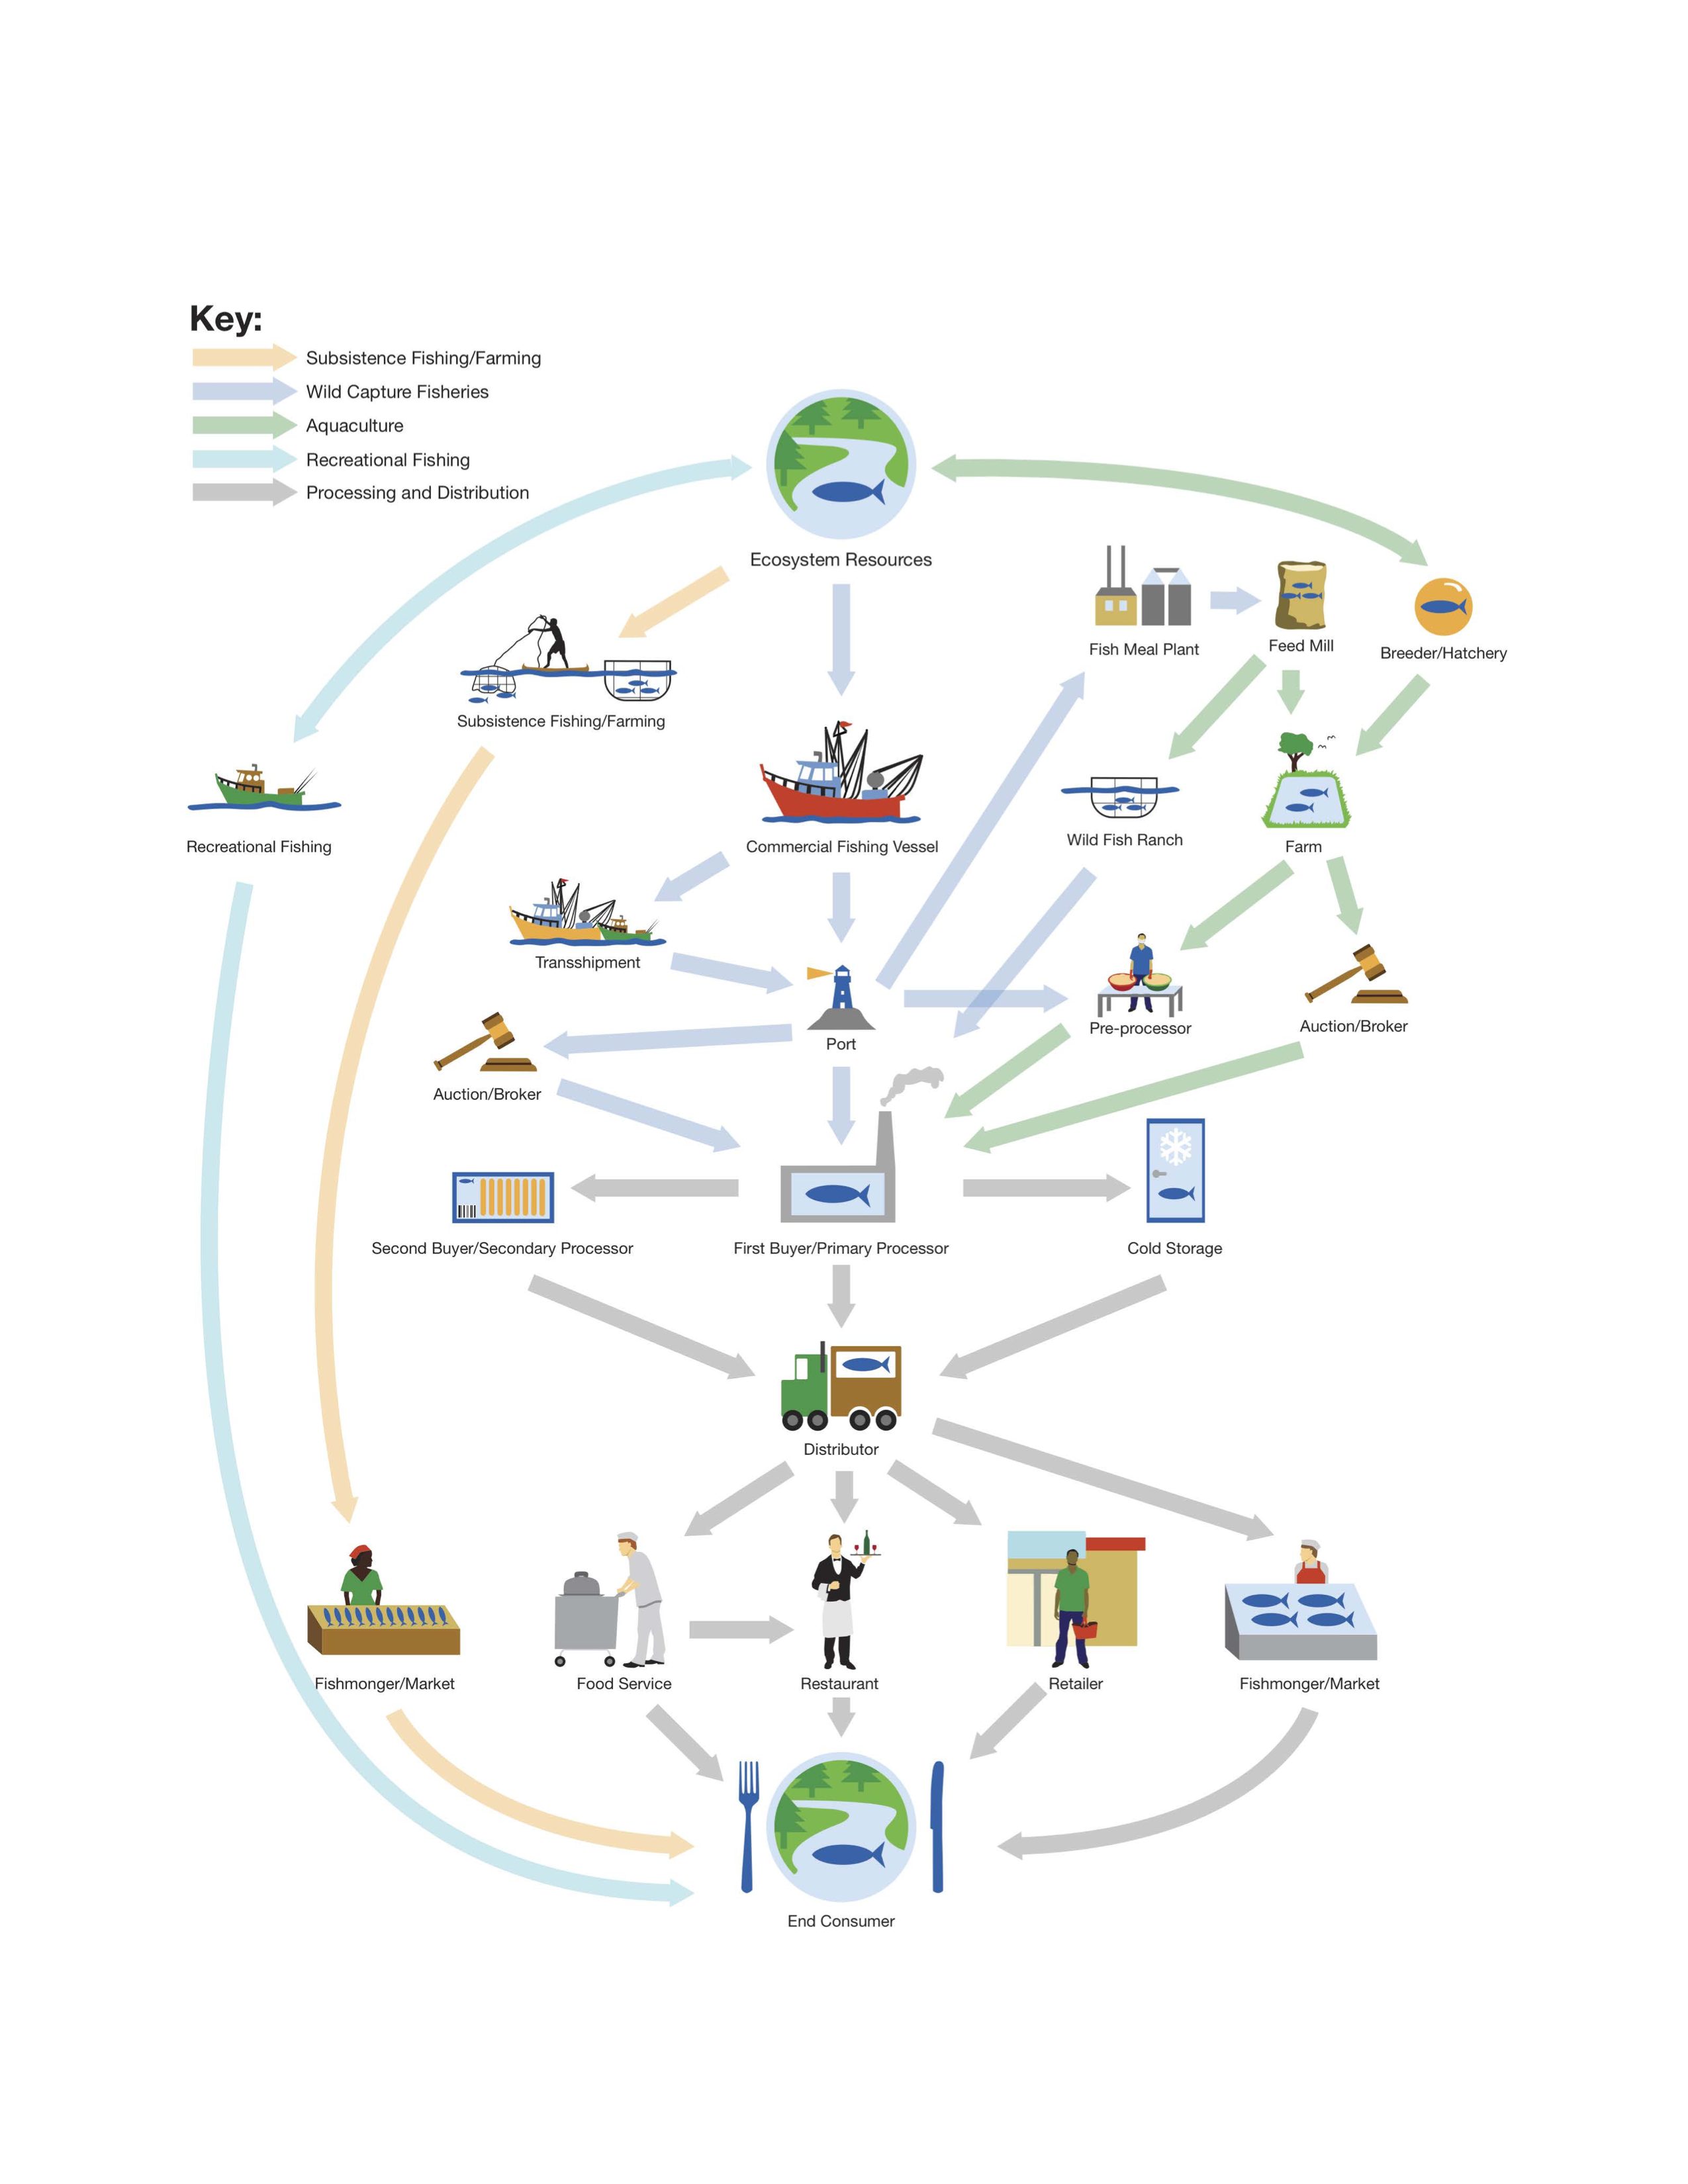
\includegraphics[height=22cm]{graphic_seafood_supply_chain.png}
%\caption{\textbf{The Complexity of the Seafood Supply Chain}}
%\emph{Source: Advancing Traceability in the Seafood Industry, FishWise}
%\end{figure}
%\newpage

\subsubsection{A seafood supply chain prototype}
A team at Intel is using \textbf{Hyperledger Sawtooth} to build a traceability prototype that combines the distributed ledger, IoT sensors, and advanced communications to track telemetry parameters throughout capture, processing, and transit. 

Sensors attached to the fish when it is caught record data such as location, temperature, and humidity. 
This data is recorded in the ledger, along with further events in the processing of the fish: ownership changes, transport company, storage temperature range, and so on. 
The ledger can also provide analytics for regulatory enforcement and scientific analysis of fish harvesting and consumption.

This prototype highlights the benefits of Hyperledger Sawtooth as a platform for tracing assets. 
The lightweight, highly decentralized consensus protocol in Sawtooth (proof of elapsed time) is particularly well-suited to a diverse, distributed ecosystem where thousands of validating nodes may be required. 
Broad participation in the ledger reflects the cross-industry nature of the seafood supply chain. 

\subsubsection{Asset tracking touches on different issues}
Asset tracking touches on several issues not generally seen in ledgers for financial products. 
For example, asset tracking requires handling diverse data types, such as the composite format required for telemetry and environmental sensing. 
Sawtooth accommodates both domain-specific data and the transaction families that operate on it, including data constraints such as verifying the calibration of a sensor.

Blockchain promises a number of benefits for cross-industry traceability. 
Most of all, these technologies can help establish a community of participants and an authoritative record of provenance. 
The blockchain's decentralized fault-tolerance enable updates from a wide range of nodes, including fishing boats, trucks, cold-storage facilities, retail stores, and restaurants. 

Beyond traceability, digitizing assets opens the door for completely new markets such as, for example, monetization of provenance.
\newpage

\section{Current Projects}
Hyperledger incubates and promotes a range of business blockchain technologies. These technologies include:  \begin{itemize}
\item Distributed ledger frameworks 
\item Smart contract engines 
\item Client libraries 
\item Graphical interfaces 
\item Utility libraries
\item Sample applications 
\end{itemize}

The Hyperledger umbrella strategy encourages the re-use of common building blocks, enables rapid innovation of components, and promotes interoperability between projects.  

Table X sums up all the current projects, in chronological order from the date they were accepted by  Hyperledger. The rest of this section sums up each project briefly, and shows where to find more information. 

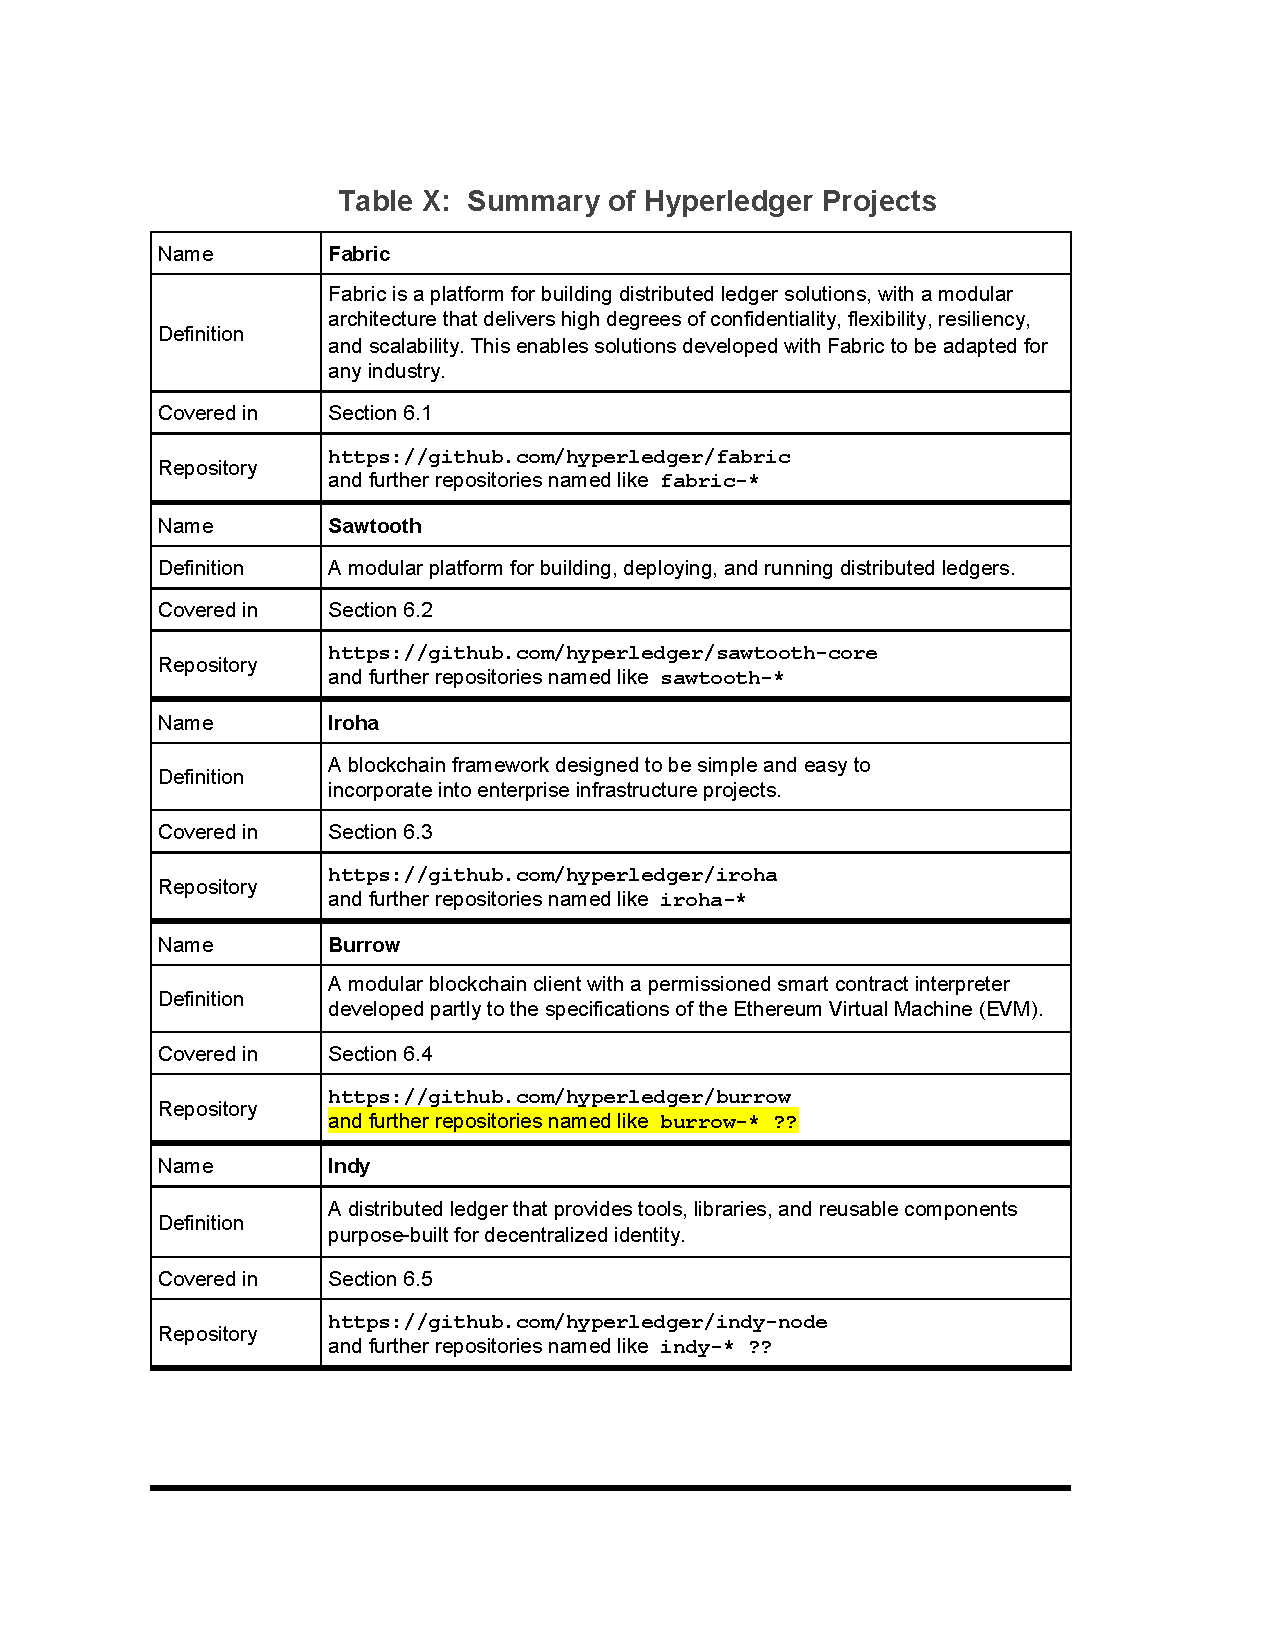
\includepdf{CurrentProjects/summary_of_hyperledger_projects_page1.pdf}

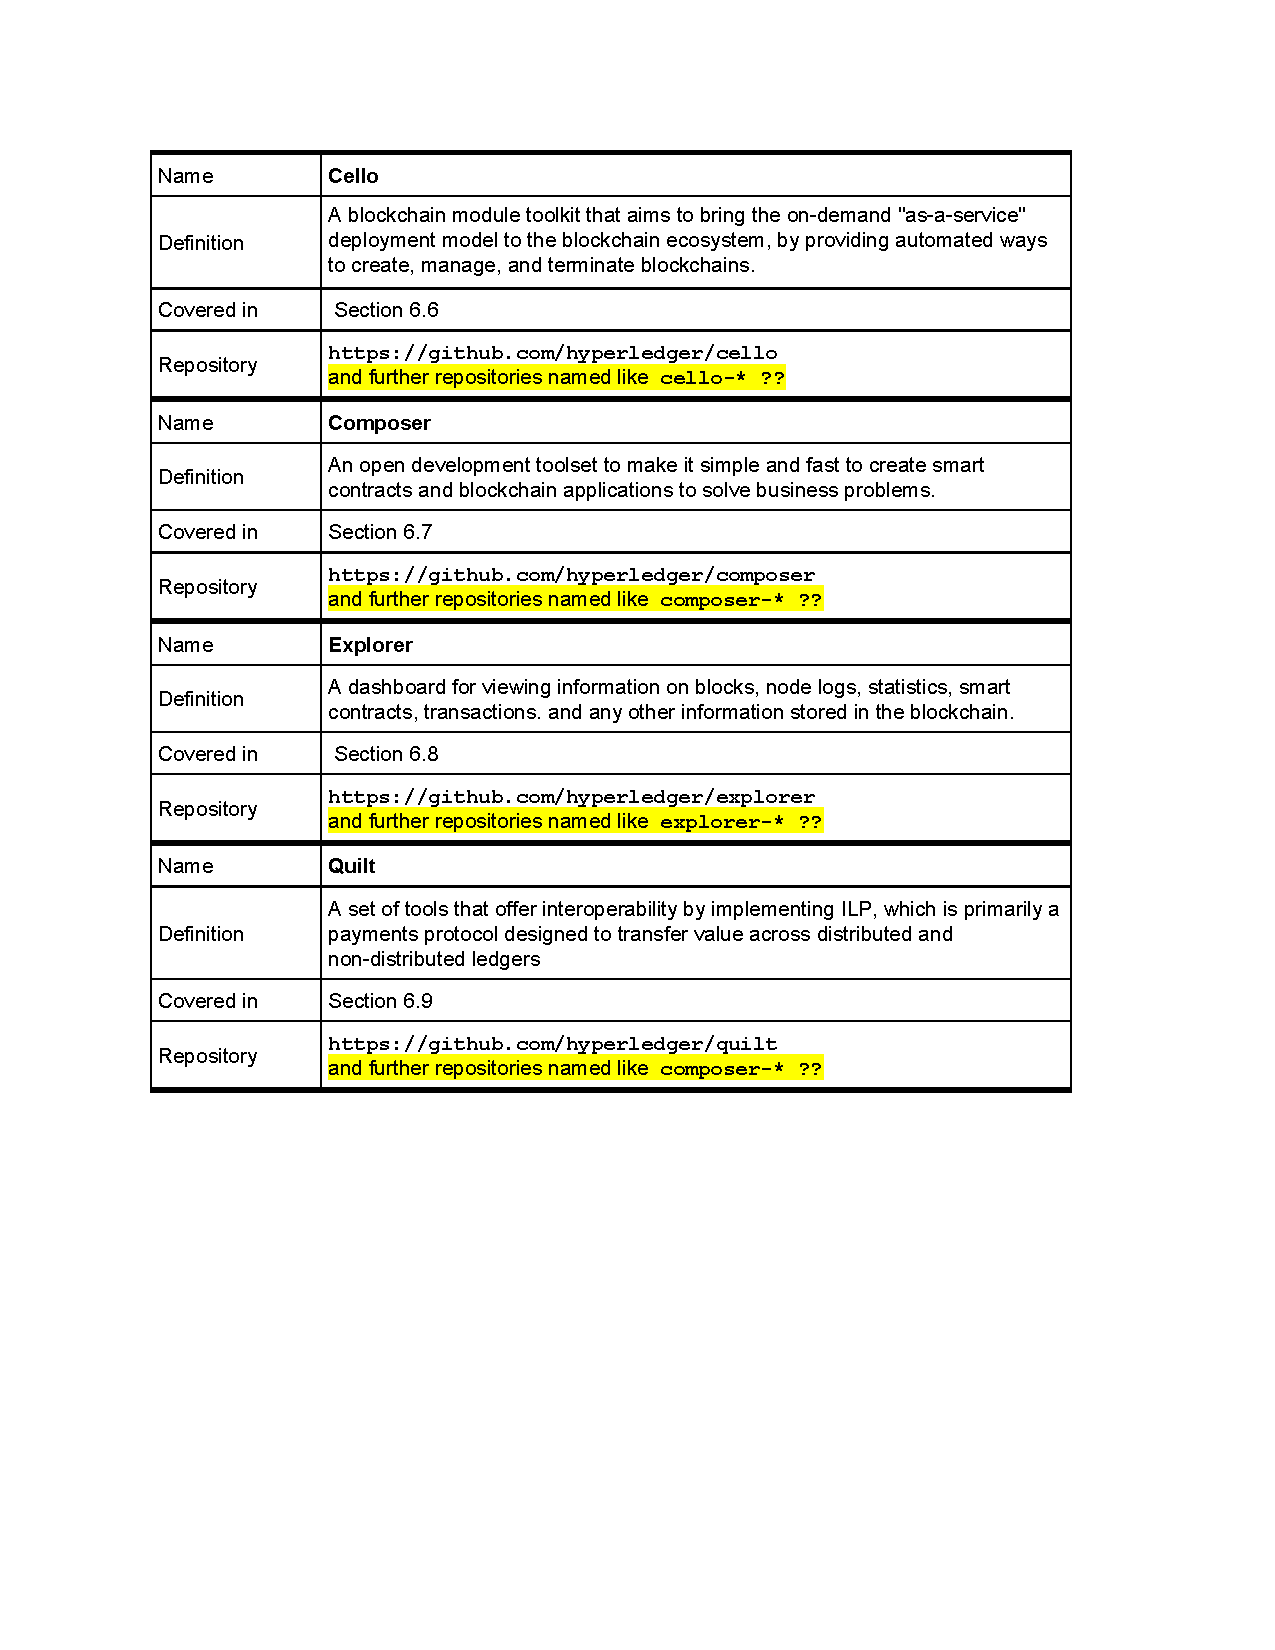
\includepdf{CurrentProjects/summary_of_hyperledger_projects_page2.pdf}
\newpage

\subsection{Hyperledger Fabric}
\textbf{Hyperledger Fabric} is a platform for building distributed ledger solutions, with a modular architecture that delivers high degrees of confidentiality, flexibility, resiliency, and scalability. 
This enables solutions developed with Fabric to be adapted for any industry. 

Fabric allows components, such as consensus and membership services, to be plug-and-play. 
It leverages container technology to host smart contracts called ``chaincode? that contain the business rules of the system. 
And it's designed to support various pluggable components, and to accommodate the complexity that exist across the entire economy.

Starting from the premise that there are no ``one-size-fits-all'' solutions, Fabric is an extensible blockchain platform for running distributed applications. 
It supports various consensus protocols, so it can be tailored to different use cases and trust models. 

Fabric runs distributed applications written in general-purpose programming languages (such as C, C++, Go,  Java, Perl, PHP, Ruby, and so on?? are these examples accurate??) without depending on any native cryptocurrency.  

This stands in sharp contrast to most other blockchain platforms for running smart contracts, which either  require code to be written in a domain-specific language or else rely on a cryptocurrency. 

Furthermore, Fabric uses a portable notion of membership for the permissioned model, which can be integrated with industry-standard identity management.  
To support such flexibility, Fabric takes a novel architectural approach and revamps the way blockchains cope with non-determinism, resource exhaustion, and performance attacks.

%Where Hyperledger Fabric breaks from some other blockchain systems is that it is private and permissioned. Rather than allowing anyone to be part of the network by either participating in the Proof-of-Work consensus or receiving transferrable forms of data such as tokens over the blockchain, the members of a Hyperledger Fabric network enroll through a membership services provider.

Fabric also supports channels, which enable a group of participants to create a separate ledger of transactions. This is especially important for networks where some participants might be competitors who don't want every transaction---such as a special price offer only to selected participants---known to every participant in the network. 
If a group of participants form a channel, only those participants and no others have copies of the ledger for that channel.

To find out more about Hyperledger Fabric, see \url{https://github.com/hyperledger/fabric} and further repositories named like \url{fabric-*}.

\subsection{Hyperledger Sawtooth}
\textbf{Hyperledger Sawtooth} is a modular platform for building, deploying, and running distributed ledgers. 
Distributed ledgers provide a digital record (such as asset ownership) that is maintained without a central authority or implementation. 
Sawtooth aims to keep distributed ledgers distributed, and to make smart contracts safe for enterprise use.
In fitting with this focus, Sawtooth is highly modular. 
This enables enterprises and consortiums to make decisions about their blockchain applications for themselves.

\subsubsection{Technical innovations in Sawtooth}
Sawtooth contains several technical innovations, including:
\begin{itemize}
\item \textbf{Unpluggable consensus}---Going beyond compile-time pluggable consensus, this allows a consortium to change consensus algorithms on a running blockchain simply by issuing a transaction.
\item \textbf{Proof of Elapsed Time (PoET)}---A consensus algorithm with the scalability of Proof of Work but without the drawback of high power consumption.
\item \textbf{Transaction families}---A smart contract abstraction that allows users to write smart contract logic in the language of their choosing.
\item \textbf{Compatability with Ethereum contracts}---Transaction families can also integrate other smart contract interpreters including Hyperledger Burrow's Ethereum Virtual Machine. 
Sawtooth features like permissioning and un-pluggable consensus enable Ethereum to be configured appropriately for an enterprise.
\item \textbf{Parallel transaction execution}---Most blockchains require transactions to be executed in series   to guarantee consistent ordering at each peer. 
Sawtooth includes an advanced parallel scheduler that splits blocks into parallel flows. 
Parallelism allows for faster block processing to partially address the performance drawback of blockchains compared to traditional databases.
\item \textbf{Private transactions}---Clusters of Sawtooth nodes can be easily deployed with separate permissioning. 
This provides privacy and confidentiality among participants of that distinct chain. 
No centralized service leak transaction patterns or other confidential information.
However, an intermediary such as \textbf{Hyperledger Quilt} is required to connect separate chains. 
In the future, Sawtooth plans to provide additional privacy and confidentiality features on top of trusted execution environments and/or zero knowledge primitives.
\end{itemize}

\subsubsection{Sawtooth extends the earlier distributed ledgers}
Originally, Sawtooth was designed to explore scalability, security, and privacy questions prompted by the earliest distributed ledgers. 
That required a modularity that was lacking at the time. 
Starting from scratch enabled the project to draw lessons from those pioneering systems, and then extend into further use cases that the original currency ledgers weren't intended to address. 

The consensus model PoET boosts scalability.
Transaction families broaden the scope of smart contracts, while narrowing the potential attack surface. 
The Sawtooth designers are also exploring trusted execution environments and the role those can play in private transactions.

Even when branching into new business cases, certain key features of a distributed ledger must be preserved. 
In an enterprise deployment, the distributed ledger must not devolve into nothing more than a replicated database. 
Enterprise participants need autonomy and have the right to run their own nodes. 

Since the set of participants will  be dynamic, the system---particularly the consensus model---must accommodate that volatility. 

\subsubsection{Over-complex and under-explained technical details}
It is not clear, for example, whether an O(n2) protocol (should we  say this, when many readers won't have a clue what this means?---GG) with fixed membership like Practical Byzantine Fault Tolerance (PBFT) can support the scale or volatility of a distributed ledger at production levels. 
It seems unwise to sidestep the challenges of providing Byzantine Fault Tolerance to operate with only a Crash Fault Tolerant consensus. 
Finally, both public and private distributed ledgers define a spectrum of authorization policies---not a binary either/or option.

To find out more about Hyperledger Sawtooth, see \url{https://github.com/hyperledger/sawtooth-core} and further repositories named like \url{sawtooth-*}.

\subsection{Hyperledger Iroha}
\textbf{Hyperledger Iroha} is a blockchain framework designed to be simple and easy to incorporate into infrastructure projects that require distributed ledger technology. 

Iroha joined Fabric and Sawtooth Lake to become the third distributed ledger platform under the Hyperledger umbrella in October, 2016. It was originally developed by Soramitsu in Japan and was proposed to Hyperledger by Soramitsu, Hitachi, NTT Data, and Colu.

Hyperledger Iroha features:
\begin{itemize}
\item A simple structure
\item Modern, domain-driven C++ design
\item Emphasis on mobile application development
\item A new, chain-based Byzantine Fault Tolerant consensus algorithm, called Sumeragi 
\end{itemize}

Iroha takes a different approach from Fabric and Sawtooth (Lake---?? GG) by providing features that are helpful for creating applications for end users. 

To find out more about Hyperledger Iroha, see \url{https://github.com/hyperledger/iroha} and further repositories named like \url{iroha-*}.

\subsection{Hyperledger Burrow}
\textbf{Hyperledger Burrow} provides a modular blockchain client with a permissioned smart contract interpreter developed partly to the specifications of the Ethereum Virtual Machine (EVM). In short, Burrow is a permissionable smart contract machine. 

Burrow became the fourth distributed ledger platform under the Hyperledger umbrella in April, 2017. 
It was originally developed and proposed to Hyperledger by Monax.

Burrow provides a strongly deterministic, smart contract-focused blockchain design. Burrow users benefit from an access control layer through the use of smart contracts and ��secure natives-based permission layer.

Burrow includes all the following components:
\begin{itemize}
\item \textbf{Consensus engine}---Maintains the networking stack between nodes and ordering transactions to be sed by the application engine.
\item \textbf{Application Blockchain Interface (ABCI)}---Provides the interface specification for the consensus engine and application engine to connect.
\item \textbf{Smart contract application engine}---Provides developers with a strongly deterministic smart contract engine for operating complex industrial processes.
\item \textbf{Gateway}---Provides programmatic interfaces for system integrations and user interfaces.
\end{itemize}

To find out more about Hyperledger Burrow, see \url{https://github.com/hyperledger/burrow}.

\subsection{Hyperledger Indy}
\textbf{Hyperledger Indy} is a distributed ledger, purpose-built for decentralized identity. 
Indy provides tools, libraries, and reusable components for creating and using independent digital identities rooted on blockchains or other distributed ledgers. 

These identities are interoperable across administrative domains, applications, and any other organizational ``silo.? Than means friends, competitors, and even antagonists can all rely on a shared source of truth. 

Indy answers fundamental questions such as, ``Who am I dealing with?" and ``How can I verify any data about the other party in this interaction?"�� 
Solid answers to these questions enable the trusted interactions that enterprises need.

\subsubsection{Key features of Indy}
\begin{itemize}
\item \textbf{Self-sovereignity}---Indy stores identity artifacts on a ledger with distributed ownership. 
These artifacts can include public keys, proofs of existence, cryptographic accumulators that enable revocation, and so on.
No one but the true owner can change or remove an identity. 
\item \textbf{Privacy}---By default, Indy preserves privacy, since every identity owner can operate without creating any correlation risk or breadcrumbs.
\item \textbf{Verifiable claims}---Identity claims can resemble familiar credentials such as  birth certificates, driver's licenses, passports, and so on. 
But these can be combined and transformed in powerful ways, using zero-knowledge proofs to enable selective disclosure of only the data required by any particular context.
\end{itemize}

\subsubsection{Many powerful benefits}
This combination of self-sovereignty, privacy, and verifiable claims is extremely powerful. 
Consider the many potential benefits. 

Bulk troves of sensitive data can vanish or become useless. 
The economics of hacking can be transformed, since less personally identifiable information (PII) is held by each business partner. 
The competing demands of preserving privacy and meeting regulations can be satisfied. 
Individuals and organizations can benefit from richer and more secure interactions. 
And the identity ecosystem can gain the innovation and dynamism of a free market. 

Despite the advanced cryptography under the hood, Indy's API is simple and straightforward. 
This API includes about 50 C-callable functions, with idiomatic wrappers for many mainstream programming languages. 

To find out more about Hyperledger Indy, see \url{https://github.com/hyperledger/indy-node} and further repositories named like \url{indy-*}.

\subsection{Hyperledger Cello}
\textbf{Hyperledger Cello} is a blockchain module toolkit that aims to bring the on-demand ``as-a-service" deployment model to the blockchain ecosystem.
The goal is to help enterprises quickly and easily adopt blockchain technologies, by providing automated ways to create, manage, and terminate blockchains. 

Cello provides an efficient and automated multi-tenant chain service on top of various infrastructures, including bare metal, virtual machine, cloud platforms like Amazon Web Services (AWS), and container platforms like Docker Swarm and Kubernetes. 
All in all, this helps boost the efficiency of ``Blockchain as a Service (BaaS)." 

Cello also provides a real-time dashboard where users can: 
\begin{itemize}
\item  View the status of the blockchain system and see statistics such as blockchain events, chaincode performance, and system utilization
\item Manage blockchains (create, configure, and delete) and chaincode (deploy and upload private chaincode)
\end{itemize}

Hyperledger Cello currently supports \textbf{Hyperledger Fabric 1.0} as the main blockchain implementation. 
The project plans to support \textbf{Sawtooth} and other types of blockchains. 

The architecture follows the micro-service style, with pluggable implementations for most components. 
The main programming languages used are Python and JavaScript.

To find out more about Cello, see  \url{https://github.com/hyperledger/cello} and further repositories named like \url{cello-*}.

\subsection{Hyperledger Composer}
\textbf{Hyperledger Composer} is an open development toolset to make it simple and fast to create smart contracts and blockchain applications to solve business problems.  
The main goal is to make it easier to integrate blockchain applications with existing business systems, and thus accelerate time-to-value. 

Composer can help develop use cases and deploy a blockchain solution in weeks, rather than months. 

With Composer, users can quickly model an existing business network, and integrate existing systems and data with blockchain applications. 
A network can contain assets---such as tangible or intangible goods, services, or property---and transactions related to them. 
As part of the model, users can define how transactions can interact wit assets. 

Business networks include the participants who interact with them. And each participant can be associated with a unique identity across several different business networks.

Hyperledger Composer supports the existing \textbf{Hyperledger Fabric} blockchain infrastructure and runtime. 
Since Fabric supports pluggable consensus protocols, this ensures that transactions can be validated according to the policy of the appropriate network participants.

To find out more about Hyperledger Composer, see \url{https://github.com/hyperledger/composer} and further repositories named like \url{composer-*}.

\subsection{Hyperledger Explorer}
\textbf{Hyperledger Explorer} provides a dashboard for viewing information about blocks, node logs, statistics, smart contracts, transactions, and any other information stored in the blockchain. 
Users can query for specific blocks or transactions to view the complete details. 

Explorer can be integrated with any authentication or authorization platforms, either commercial or open source, to provide the functions appropriate to the user's privileges. 

The goals of the Explorer project include:
\begin{itemize}
\item To create a web application for a generic blockchain explorer that's easy to install and can be used with different blockchain platforms
\item To use the latest tools and technologies to make Explorer easy to implement, maintain, and extend
\item To support the standard package managers available on most popular platforms to ensure the Explorer is quick and easy to install
\end{itemize}

To find out more about Hyperledger Explorer,  see \url{https://github.com/hyperledger/blockchain-explorer} and further repositories named like \url{explorer-*}.

\subsection{Hyperledger Quilt}
\textbf{Hyperledger Quilt} offers interoperability between ledger systems by implementing Interledger Protocol (ILP), a payments protocol designed to transfer value across both distributed and non-distributed ledgers. 

At publication date, Hyperledger Quilt was coming soon. 

\subsubsection{About the ILP}
Payment networks today are siloed and disconnected. 
Payments are relatively easy within one country, or if both the sender and recipient have accounts on the same network or ledger. 
But sending from one ledger to another is often impossible. 
Where connections do exist, they are manual, slow, or expensive.

The Interledger Protocol provides for routing payments across different digital asset ledgers, while isolating senders and receivers from the risk of intermediary failures. 
Secure multi-hop payments and automatic routing enable a global network of networks for different types of value that can connect any sender with any receiver.

\subsubsection{For more information}
To find out more about ILP, visit \url{https://interledger.org/rfcs/0003-interledger-protocol/}.

To see more about Hyperledger Quilt, visit the Projects webpage at \url{https://www.hyperledger.org/projects#}.

%\Or see \url{https://github.com/hyperledger/quilt} and further repositories named like \url{quilt-*}. 
\newpage

\section{Long-Term Vision}
We live in a highly interconnected world. 
In the future, the world will no doubt become even more closely tied together.
In both our business and personal lives, more data, more digital content, more communication, and more sharing will be the norm. 
All this will require careful management of our security, privacy, and trust. 

\subsection{A common problem, and a sensible solution}
We expect to see a common problem: Many people will want to share data in a distributed database, but no single owner will be trusted by every user. 

The solution is distributed ledger technology (DLT). 
As data sharing increases, we expect blockchain technology and DLT to become more and more common.

But reaching widespread use of distributed ledgers will not be simple. 
For instance, gaining security and privacy with a blockchain often means sacrificing  performance. 
This suggests that we'll need a variety of different blockchains that can all communicate and interact seamlessly.
No one blockchain will work best for all applications.

The long-term vision for Hyperledger is driven by two main concerns: that the architecture must be modular and interoperable.

\subsection{Interchangeable modules}
We hope that eventually Hyperledger consists of many modules that can be assembled into a cohesive, functional, and secure distributed ledger. 
All these modules must be interchangeable with other modules of the same type. 
All modules must be able to communicate with other modules of the same or different types. 
And ideally, even a non-expert will be able to use them to set up a secure, interoperable blockchain quickly, easily, and efficiently.

\subsection{Many blockchains that work together}
We want to specifically point out that we do not believe any Hyperledger blockchain should be the ``one distributed ledger to rule them all.'' 
The Hyperledger community sees merit in many different blockchains. 
We hope that other developers consider interoperability with Hyperledger projects. 

\subsection{Not a single stack, but a collection of tools}
The goal for Hyperledger is not to become a single software stack. 
Instead, we want to create a collection of tools built with modularity and interoperability in mind. 
Then, any individual can use one, some, or all of the Hyperledger projects to create a distributed ledger to suit their needs.

In the future, we hope that Hyperledger can solve most of the common problems in the distributed ledger space. 
This will require a good community of developers, strong support from business and industry, and solid design principles. 
As shown in this paper, we have structured Hyperledger with all these in mind. 
\newpage

\section{Conclusions}
In this paper, we explained the rationale behind the creation of Hyperledger and our goals for the project. 
We outlined why we think an open source umbrella organization seems to be the optimal governing arrangement for a general blockchain consortium.
We showcased some of the many use cases that inspired our members to join and work on Hyperledger.
We described some of the features required to build effective blockchains for some of these use cases. 
And we briefly summed up all the Hyperledger projects and where they stand at publication date. 

We hope reading this paper is just the beginning of the Hyperledger experience for you. 

We know there's a lot of work left to be done.
We realize that Hyperledger will probably always be a work-in-progress. 
But---perhaps with your help--we can all work together to build secure, efficient, and reliable blockchain solutions that make a difference to everyone's future.

\subsection{Introductory Sources on Blockchain}
~\newline
\emph{Blockchain Technology Overview}. National Institute of Standards and Technology, U.S. Department of Commerce. January 2018. One of the best introductions to blockchain we have seen, written in plain English while maintaining nuances. Includes glossary of terms and acronyms. 
~\newline
~\newline
\emph{Blockchain Basics: Glossary and use cases}. IBM developer-Works. Updated August 21, 2017. A solid explanation of blockchain terms aimed at developers new to the space. 
~\newline
~\newline
\emph{Blockchain Basics: A Non-Technical Introduction in 25 Steps}. Daniel Drescher. Apress. March 2017. Explains blockchain concepts with analogies, metaphors, and pictures, not mathematical formulas or program code. (\emph{GG ordered but hasn't received it yet, supposed to be good explanations in plain English...})
~\newline
~\newline
\emph{Blockchain Revolution: How the Technology Behind Bitcoin Is Changing Money, Business, and the World}. Don Tapscott and Alan Tapscott. Portfolio--Penguin. May 2016. Less about the technology and more about the implications of blockchain for business. The authors also have basic videos available on YouTube. 

\subsection{Further Resources from Hyperledger}
We encourage you to use the Hyperledger resources to find more information on any blockchain-related topics you find interesting. Here are some further resources to get you started. 

\emph{The Hyperledger Vision} is a slide deck that sums up some blockchain 101-type information and the founding vision for Hyperledger, available at \url{https://www.hyperledger.org/resources/publications}. 
 
\emph{The Hyperledger Wiki} contains a wealth of technical information, available at \url{https://wiki.hyperledger.org/start}.

Each of the main projects under Hyperledger is working on a \emph{Getting Started} guide and has further information available at these links:
\begin{itemize}
\item Fabric---\url{https://www.hyperledger.org/projects/fabric}
\item Sawtooth---\url{https://www.hyperledger.org/projects/sawtooth}
\item Iroha---\url{https://www.hyperledger.org/projects/iroha}
\item Burrow---\url{https://www.hyperledger.org/projects/hyperledger-burrow}
\item Indy---\url{https://www.hyperledger.org/projects/hyperledger-indy}
\item Cello---\url{https://www.hyperledger.org/projects/cello}
\item Composer---\url{https://www.hyperledger.org/projects/composer}
\item Explorer---\url{https://www.hyperledger.org/projects/explorer}
\item Quilt---coming soon \url{}
\end{itemize} 

The Hyperledger Working Groups have many great technical resources, and are open to anyone with an interest in their subjects.  For example, the Architecture Working Group has substantial documentation on the fundamentals of permissioned blockchain. If you're looking to explore technical details, that group is a great resource. 

The application-specific working groups are also great places to learn. For instance, the Identity Working Group has spent a lot of time discussing and documenting how blockchain can enable identity solutions. 

%\iftoggle{fullversion}{
 %   \bibliographystyle{alpha}
%}{
 %   \bibliographystyle{alpha}
%}
%\bibliography{hyperledger}

\end{document}
